% Copyright 2004 by Till Tantau <tantau@users.sourceforge.net>.
%
% In principle, this file can be redistributed and/or modified under
% the terms of the GNU Public License, version 2.
%
% However, this file is supposed to be a template to be modified
% for your own needs. For this reason, if you use this file as a
% template and not specifically distribute it as part of a another
% package/program, I grant the extra permission to freely copy and
% modify this file as you see fit and even to delete this copyright
% notice.
\documentclass[notes]{beamer}
% There are many different themes available for Beamer. A comprehensive
% list with examples is given here:
% http://deic.uab.es/~iblanes/beamer_gallery/index_by_theme.html
% You can uncomment the themes below if you would like to use a different

%\usetheme{AnnArbor}
%\usetheme{Antibes}
%\usetheme{Bergen}
%\usetheme{Berkeley}
%\usetheme{Berlin}
%\usetheme{Boadilla}
%\usetheme{boxes}
%\usetheme{CambridgeUS}
%\usetheme{Copenhagen}
%\usetheme{Darmstadt}
%\usetheme{default}
%\usetheme{Frankfurt}
%\usetheme{Goettingen}
%\usetheme{Hannover}
%\usetheme{Ilmenau}
%\usetheme{JuanLesPins}
%\usetheme{Luebeck}
%\usetheme{Madrid}
%\usetheme{Malmoe}
%\usetheme{Marburg}
%\usetheme{Montpellier}
%\usetheme{PaloAlto}
%\usetheme{Pittsburgh}
%\usetheme{Rochester}
%\usetheme{Singapore}
%\usetheme{Szeged}
%\usetheme{Warsaw}
%\usetheme[]{metropolis}

\title{A Lagrangian geography of the deep\\Gulf of Mexico}

% A subtitle is optional and this may be deleted
%\subtitle{Optional Subtitle}

\author{Philippe Miron\inst{1},  Francisco J. Beron-Vera\inst{1}, Mar\'ia J. Olascoaga\inst{1}, Gary Froyland\inst{2}, J.\ Sheinbaum\inst{3} and P.\ P\'erez-Brunius\inst{3}}
\institute
{
  \inst{1}%
  RSMAS University of Miami, Miami, USA
  \and
  \inst{2}%
  University of New South Wales, Sydney, Australia
  \and
  \inst{3}
  CICESE, Ensenada, Mexico
  
  }
% - Use the \inst command only if there are several affiliations.
% - Keep it simple, no one is interested in your street address.

\date{Ocean Sciences Meeting on Wednesday, February 14 2018}
% - Either use conference name or its abbreviation.
% - Not really informative to the audience, more for people (including
%   yourself) who are reading the slides online

\subject{Applied oceanography}
% This is only inserted into the PDF information catalog. Can be left
% out. 

% Beamer settings
\setbeamertemplate{navigation symbols}{} %remove nav symbols
\setbeamertemplate{bibliography item}{}
\setbeamertemplate{footline}[frame number]

% If you have a file called "university-logo-filename.xxx"
% is a graphic format that can be processed by latex or pdflatex,
% resp., then you can add a logo as follows:
%\pgfdeclareimage[height=1.5cm]{logo}{figures/GoMRi.png}
%\logo{\pgfuseimage{logo}}

% Delete this, if you do not want the table of contents to pop up at
% the beginning of each subsection:
%\AtBeginSubsection[]
%{
%  \begin{frame}<beamer>{Outline}
%  \tableofcontents[currentsection,currentsubsection]
%  \end{frame}
%}

% graphic
\graphicspath{{"2018. deep floats (agu)/figures/"}}
%\graphicspath{{"figures/"}}

% titlepage logo
\titlegraphic{
\begin{tikzpicture}[overlay, remember picture]
%\node[at=(current page.south west), anchor=south west] {%
% 
\includegraphics[height=.10\textwidth]{carthe.png} 
%};
\node[at=(current page.south west), anchor=south west] {%
 
\includegraphics[height=.18\textwidth]{cigom.jpg} 
};
\node[at=(current page.south east), anchor=south east] {
 
\includegraphics[height=.14\textwidth]{um-rsmas.png}
};
\end{tikzpicture}
}

% bibliography
\usepackage[style=authoryear, natbib=true]{biblatex}
\addbibresource{oce.bib}
% remove annoying biblatex bug/warning
\usepackage{silence}
\WarningFilter{biblatex}{Patching footnotes failed}

% some definitions
\usepackage[utf8]{inputenc}
\usepackage[english]{babel}
\usepackage{amssymb}
\usepackage{amsfonts}
\usepackage{amsmath}
\usepackage{bbold}
\usepackage{ragged2e} % justify text in all frame
\apptocmd{\frame}{}{\justifying}{}
\usepackage{etoolbox}
\usepackage{tikz}
\usepackage{subfig}
\usepackage{multicol}
\usepackage{siunitx}
\usepackage{csquotes}
\usepackage{hyperref}
\usepackage{tikz,pgfplots}
\pgfplotsset{compat=1.12}

% Definitions.
\DeclareMathOperator{\area}{area}%
\DeclareMathOperator{\Id}{Id}%
\newcommand{\PF}{\mathcal{P}}
\newcommand{\ia}{\textit{a}}
\newcommand{\ib}{\textit{b}}
\newcommand{\ic}{\textit{c}}
\newcommand{\id}{\textit{d}}
\newcommand{\ie}{\textit{e}}
\newcommand{\gom}{GoM}
\let\vaccent=\v 
\renewcommand{\v}[1]{\ensuremath{\mathbf{#1}}} 
\newcommand{\minus}{\scalebox{0.5}[1.0]{$-$}}
\newcommand{\dif}{\ensuremath{\text{d}}}

% Let's get started
\begin{document}

\frame[plain,noframenumbering]{
\titlepage
}

\iffalse
\begin{frame}{Outline}
  \tableofcontents
  % You might wish to add the option [pausesections]
\end{frame}
\fi

\section{Introduction}

\iffalse
\frame{\frametitle{Introduction}
Over the last twenty five years, many satellite-tracked surface drifters sampled the surface of the Gulf of Mexico (\gom). From a database of 3300 drifters, we presented a Lagrangian geography of the \gom.

\begin{figure}
    \centering
    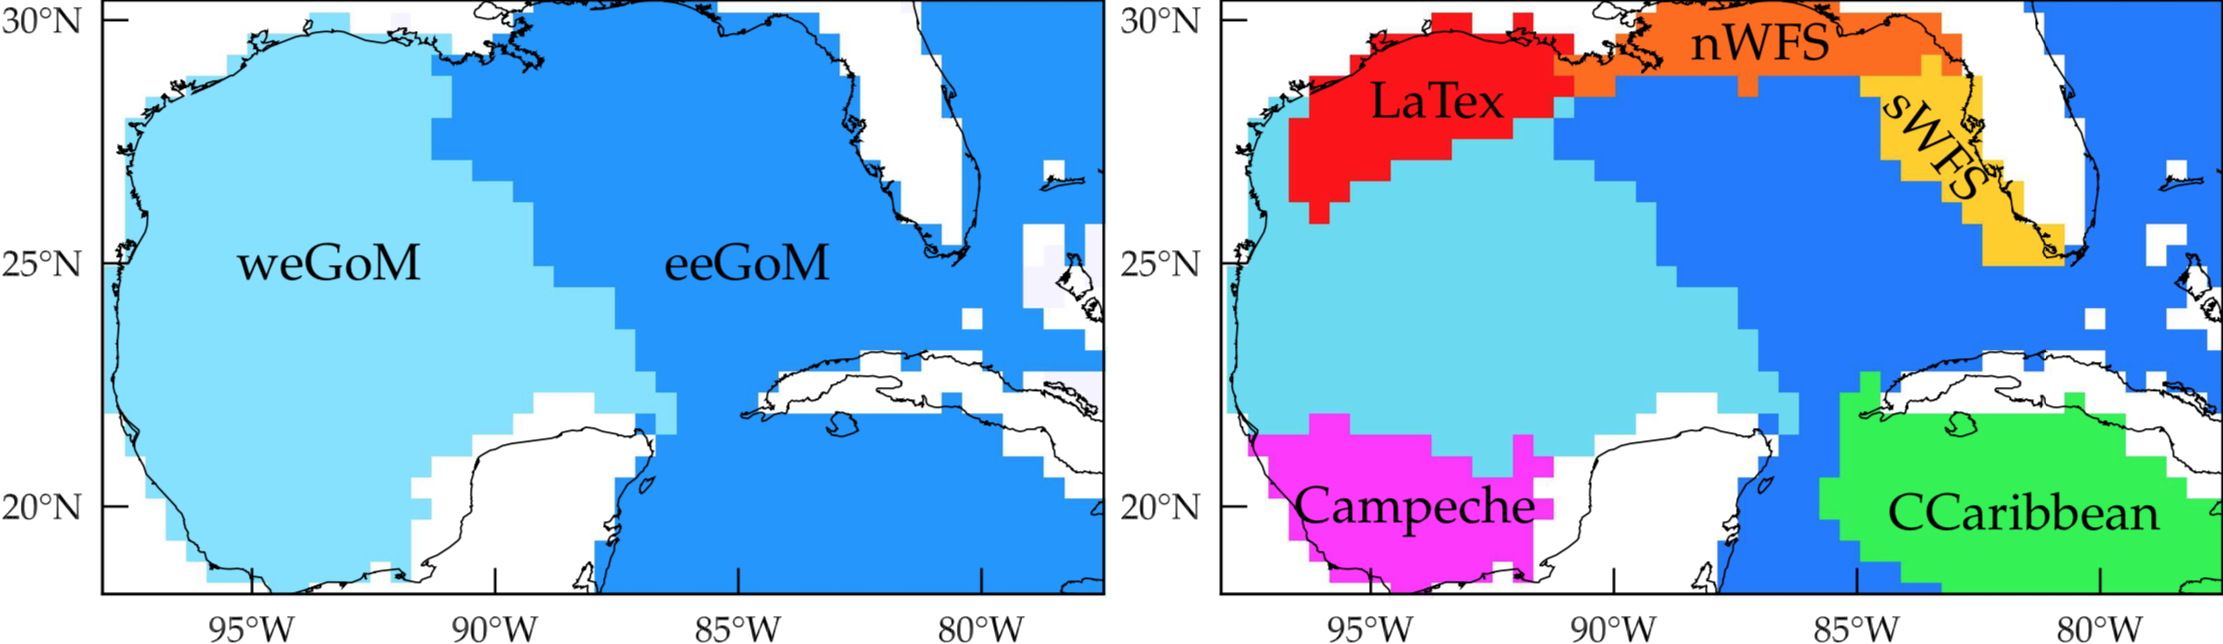
\includegraphics[width=\textwidth]{geosurf.png}
    \caption{Published in \cite{miron2017lagrangian}}
    \label{fig:geosurf}
\end{figure}
}
\fi

\frame{\frametitle{Introduction}
RAFOS experiment sponsored by the Bureau of Ocean Energy Management (July 2011 - May 2015)\footnote{Publicly available data sets compiled by WOCE Subsurface Float Data Assembly Center (WFDAC).}:
\begin{itemize}
\item 4-year-long program (floats $\sim 2$-y mission)
\item 121 floats at 1500\,m
\item 6 profiling floats with RAFOS technology at 1500\,m
\item 31 floats at 2500\,m
\end{itemize}

\begin{figure}
    \centering
    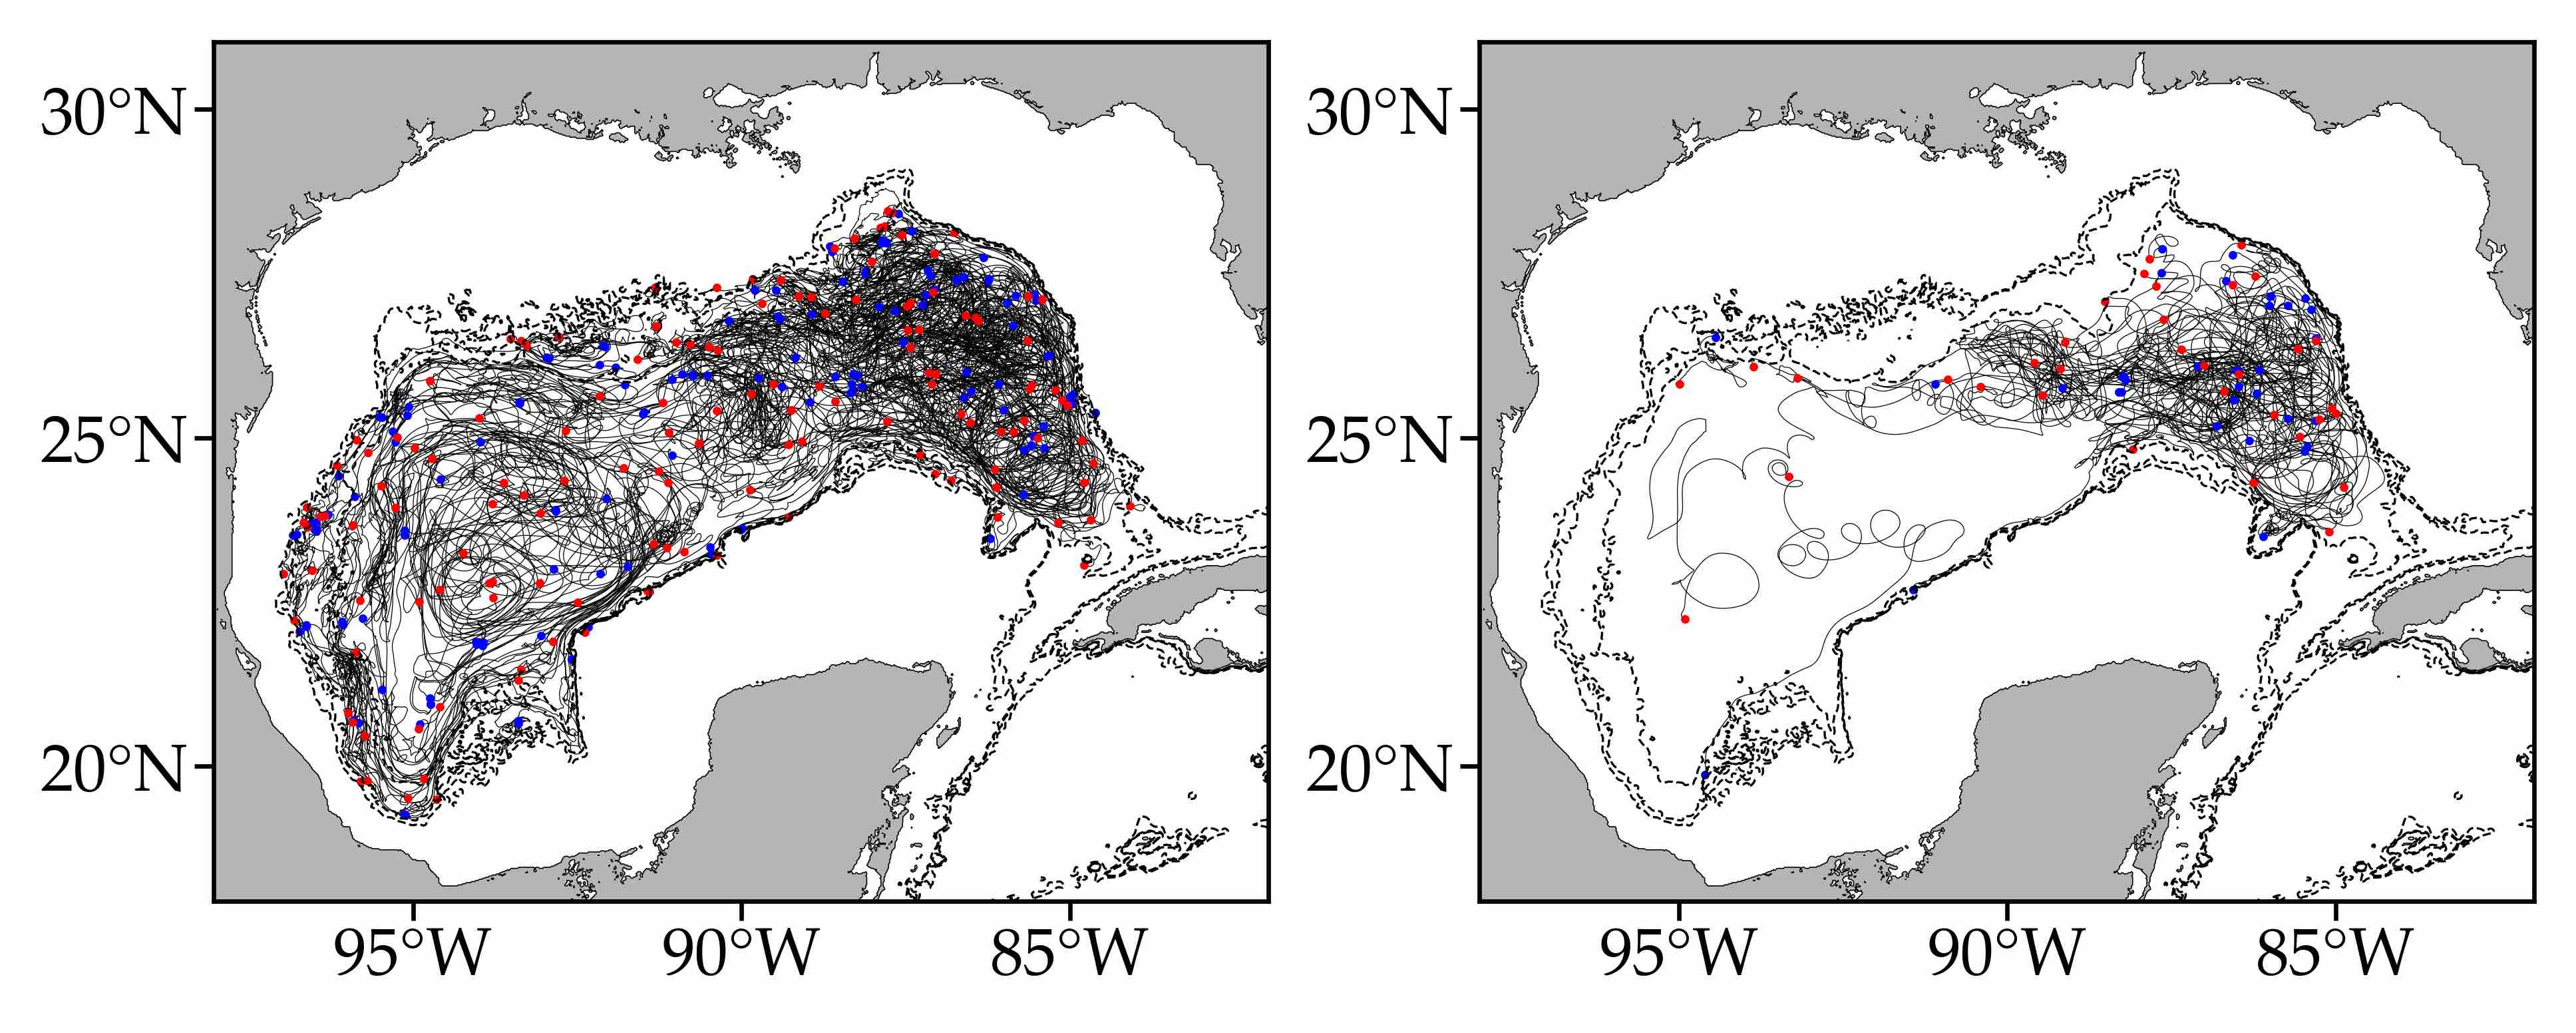
\includegraphics[width=\textwidth]{geogomdeep-fig01}
\end{figure}

}

\section{Objectives}

\frame{\frametitle{Objectives}
Using floats data (trajectories) in the abyssal Gulf of Mexico (\gom):
\begin{itemize}
    \item subdivide the deep \gom\ into regions with similar dynamics;
    \item identify almost invariant regions and their respective timescale;
    \item assess connectivity.
\end{itemize}
}

\frame{\frametitle{Seasonality of the RAFOS Data}

The data coverage isn't sufficient for full seasonal analysis but assuming time homogeneity it is enough to build a Markov-Chain model \citep{maximenko2012pathways,miron2017lagrangian,mcadam2018surface}.
\begin{figure}
    \centering
    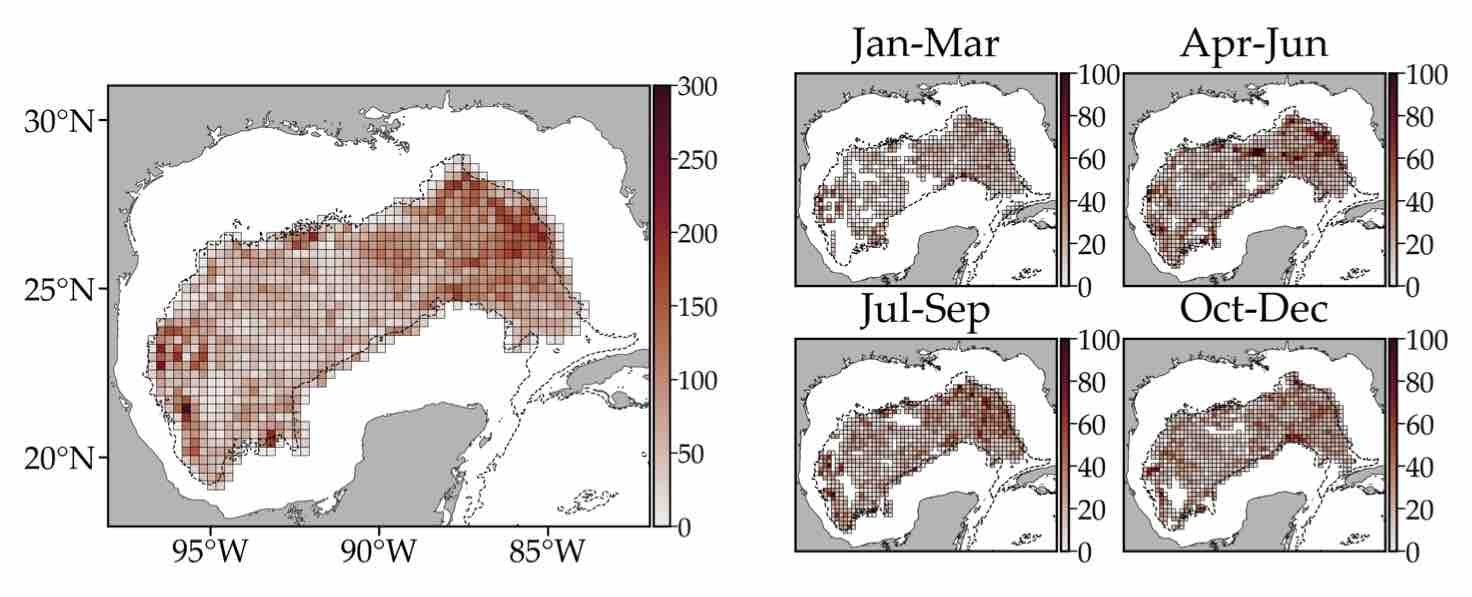
\includegraphics[width=\textwidth]{geogomdeep-fig02}
\end{figure}
}

\iffalse
\frame{\frametitle{Theory: transfer operator $\mathcal{P}$}
We want to predict at a time $T$ the dispersion of a initial density $\rho(x,0) = f(x)$.
\begin{itemize}
    \item using data from float trajectories;
    \item not using directly a advection-diffusion equation;
    \item model by a stochastic kernel $k$ that gives probability to move from one part of the domain to the other;
    \item not model as function of initial time.
\end{itemize}

\begin{equation}
     \mathcal{P}\,f(x) = \int_X k(x,y)\, f\dif y = \rho(x,T),
\end{equation}
}
\fi

\iffalse
\frame{\frametitle{Theory: how to construct the transition matrix}

\begin{itemize}
    \item A discretization of the transfer operator is obtained using a Galerkin approximation;
    \item involves partitioning the domain $X$ into a grid of $N$ regular connected boxes $\{B_1,\dotsc,B_N\}$
    \item projecting functions in $L^1(X)$, the space of absolutely integrable functions, onto a finite-dimensional space spanned by indicator functions on the grid.
\end{itemize}
}
\fi

\frame{\frametitle{Theory: how to construct the transition matrix}  

By partitioning the domain $X$ into a grid of $N$ regular connected boxes $\{B_1,\dotsc,B_N\}$ and with large number of initial conditions we can estimate the entries:
\begin{equation}
   \mathcal{P} \approx P_{ij} = \frac{\# x \text{ in }B_i\text{ at any time } t \text{ and in }B_j \text{ at  } t+T}{\#x\text{ in }B_i \text{ at any time }t},
  \label{eq:Pnum}
\end{equation}
which are transitional probabilities of moving from $B_i$ to $B_j$. It defines a \textbf{Markov Chain} (with bins $\equiv$ states) of the dynamics.
\newline\newline
Timescale T is fix at 7-d which is larger then the decorrelation scale of 5-d and enough to allow interbins connection.
}

\frame{\frametitle{Application of the transition matrix}
One can push forward discrete representations of $f(x)$:
\begin{equation}
    \mathbf f = (f_1,\cdots,f_N),
\end{equation}
under left-multiplication by $P$:
\begin{align}
    f^{(1)} &= f\,P \nonumber\\
    f^{(2)} &= f^{(1)}\,P = f\,P^2 \nonumber\\
    f^{(k)} &= f\,P^k
\end{align}
}

\frame{\frametitle{Eigenvectors analysis}

It is also of interest to identify when a distribution $\mathbf f$ is almost invariant:
\begin{equation}
    \mathbf f \approx \mathbf f\,P
\end{equation}

This is available from the \emph{eigenspectrum} inspection of $P$ \citep{Froyland-etal-12}.
\newline\newline
If in the matrix $P$:
\begin{itemize}
    \item all states \emph{communicate};
    \item no state occurs \emph{periodically}.
\end{itemize}
$P$ has one $\lambda = 1$ a limiting distribution $\mathbf{p} = \mathbf{p} P$.
\newline\newline
Note: $\mathbf{p}$ is a left eigenvector of $P$ (row-stochastic matrix) with eigenvalue $\lambda = 1$.
\begin{align*}
    \mathbf{p} \lambda &= \mathbf{p} P\\
    \mathbb{1} \lambda &= P\mathbb{1}
\end{align*}
}

\frame{\frametitle{Attractors and basin off attractions}

Motivates the idea that regions where trajectories converge and their basins of attraction are encoded in the eigenvectors of the transition matrix $P$ with eigenvalues ($\lambda \approx 1$) \citep{froyland2014well}.

\begin{itemize}
    \item \textbf{right eigenvector} of $P$ is the basin of attraction (\textbf{constrains connectivity!})
    \item \textbf{left eigenvector}  of $P$ is the attractor or almost-invariant region
\end{itemize}
}

\section{Results}
\frame{\frametitle{Eigenvectors}

\only<1>{
Eigenvectors associated with $\lambda_1=1$ and $\lambda_2=0.9953$.
\begin{figure}
  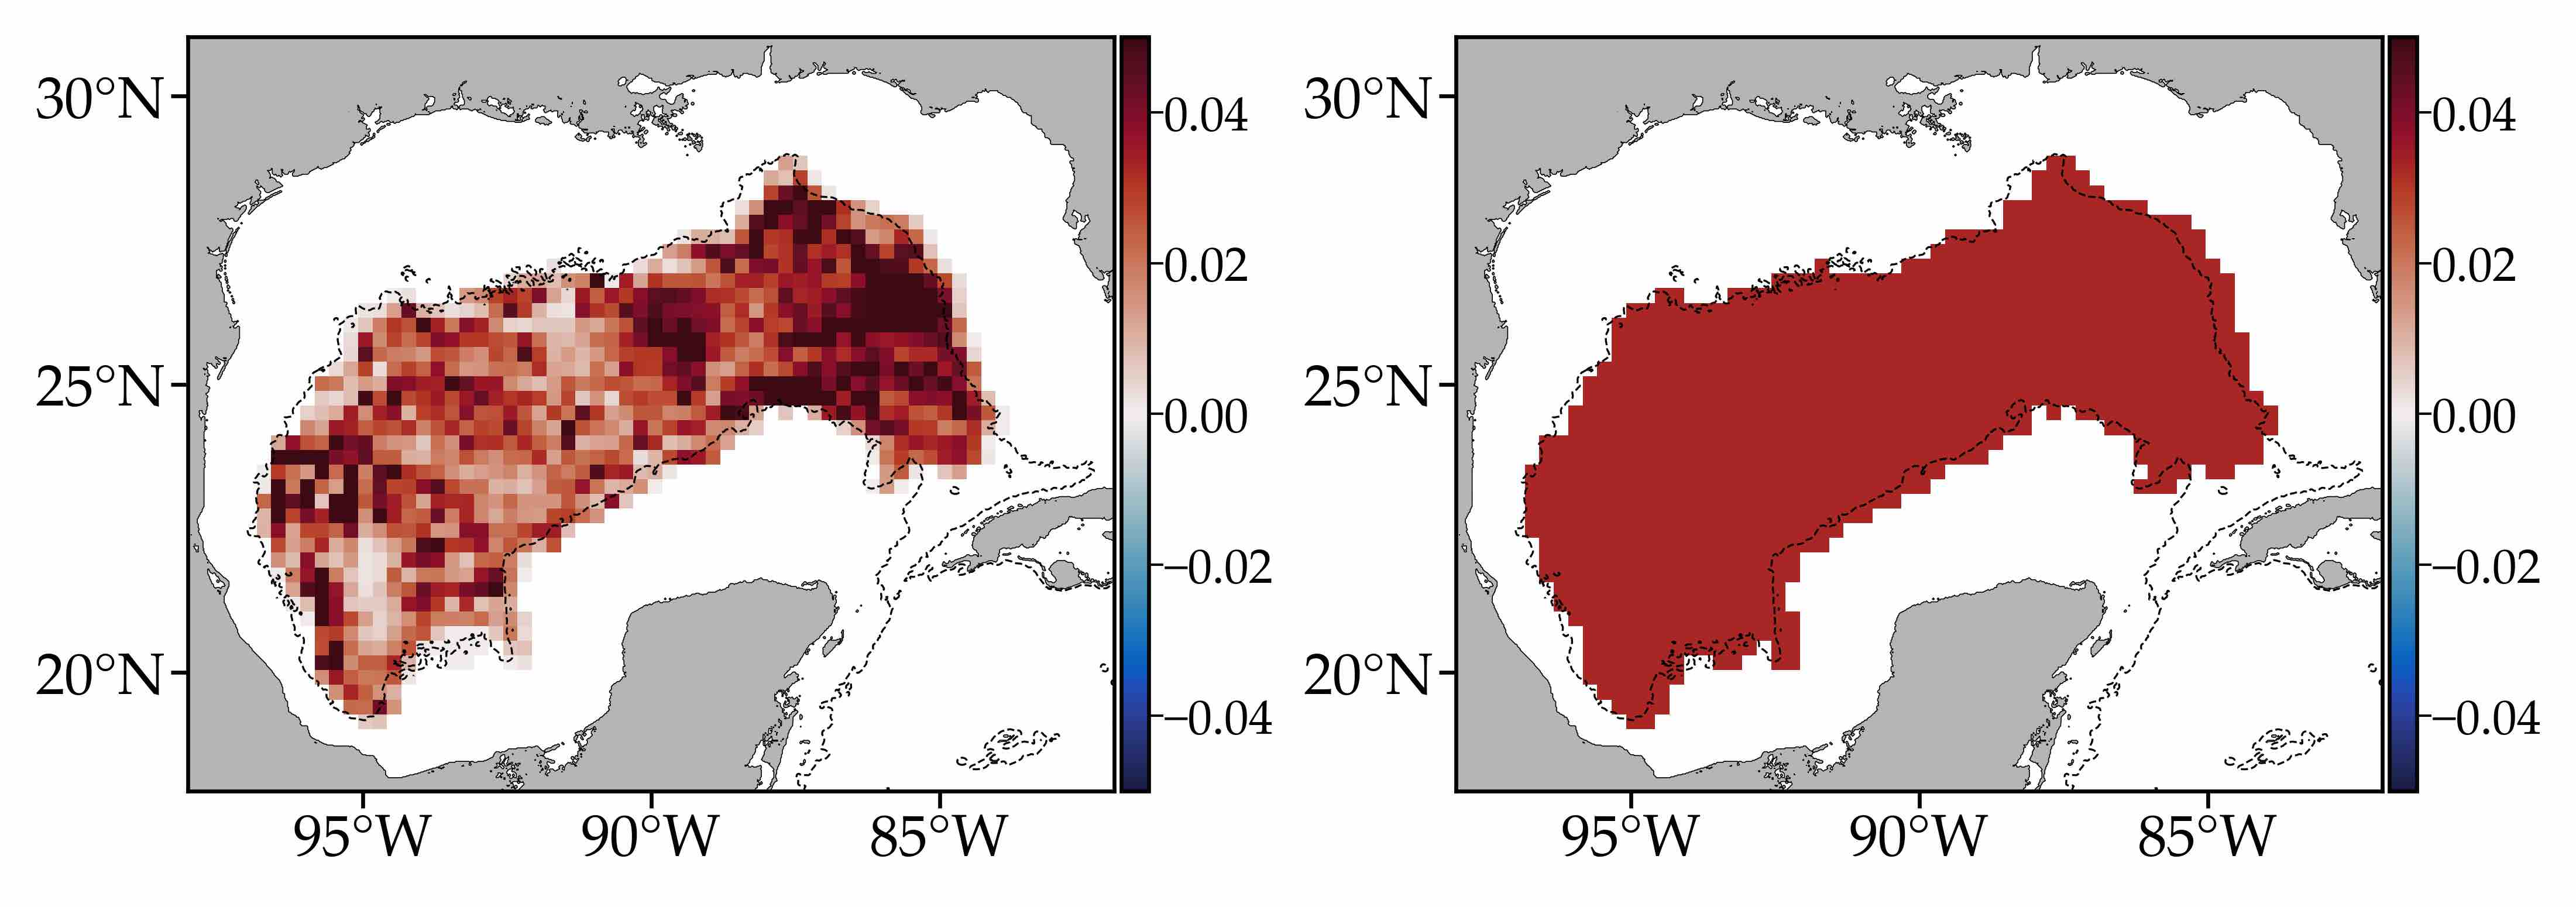
\includegraphics[width=\textwidth]{geogomdeep-fig07.jpg}
\end{figure}
\begin{figure}
  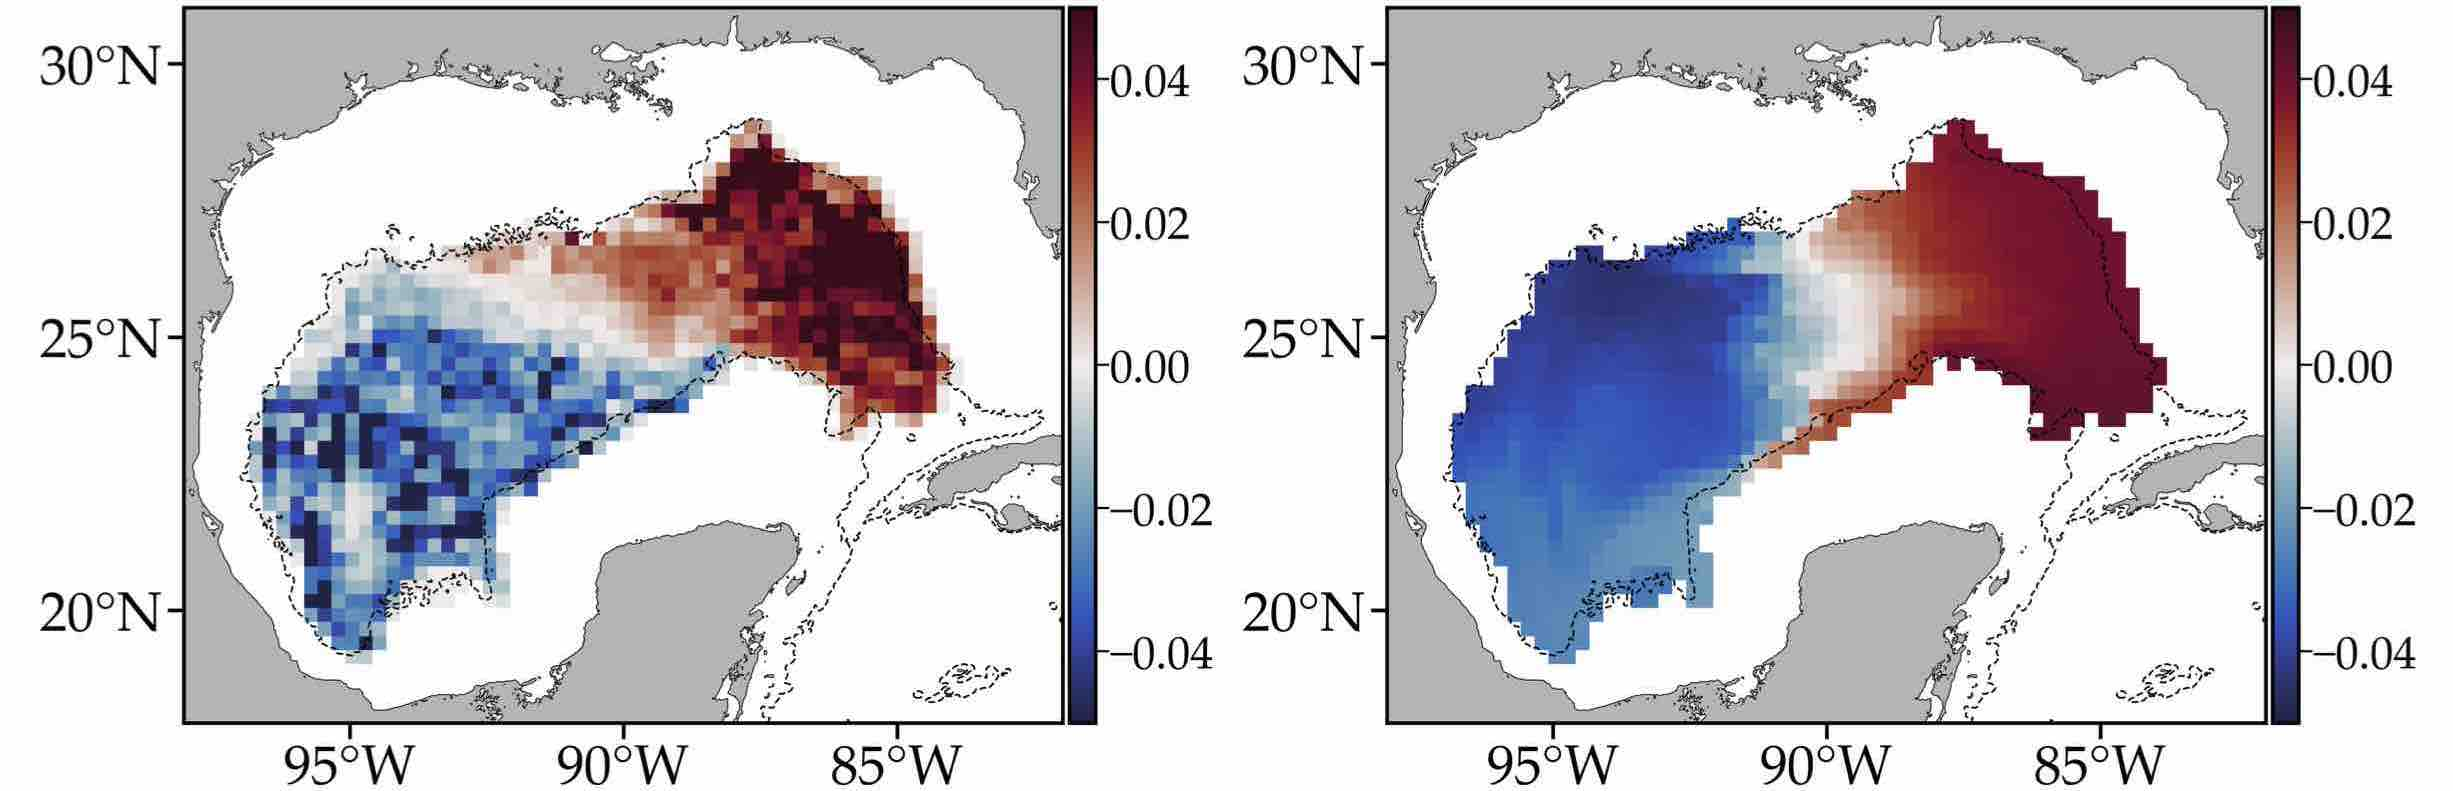
\includegraphics[width=\textwidth]{geogomdeep-fig08a.jpg}
\end{figure}
}

\only<2>{
Eigenvectors associated with $\lambda_3=0.9832$ and $\lambda_5=0.9712$.
\begin{figure}
  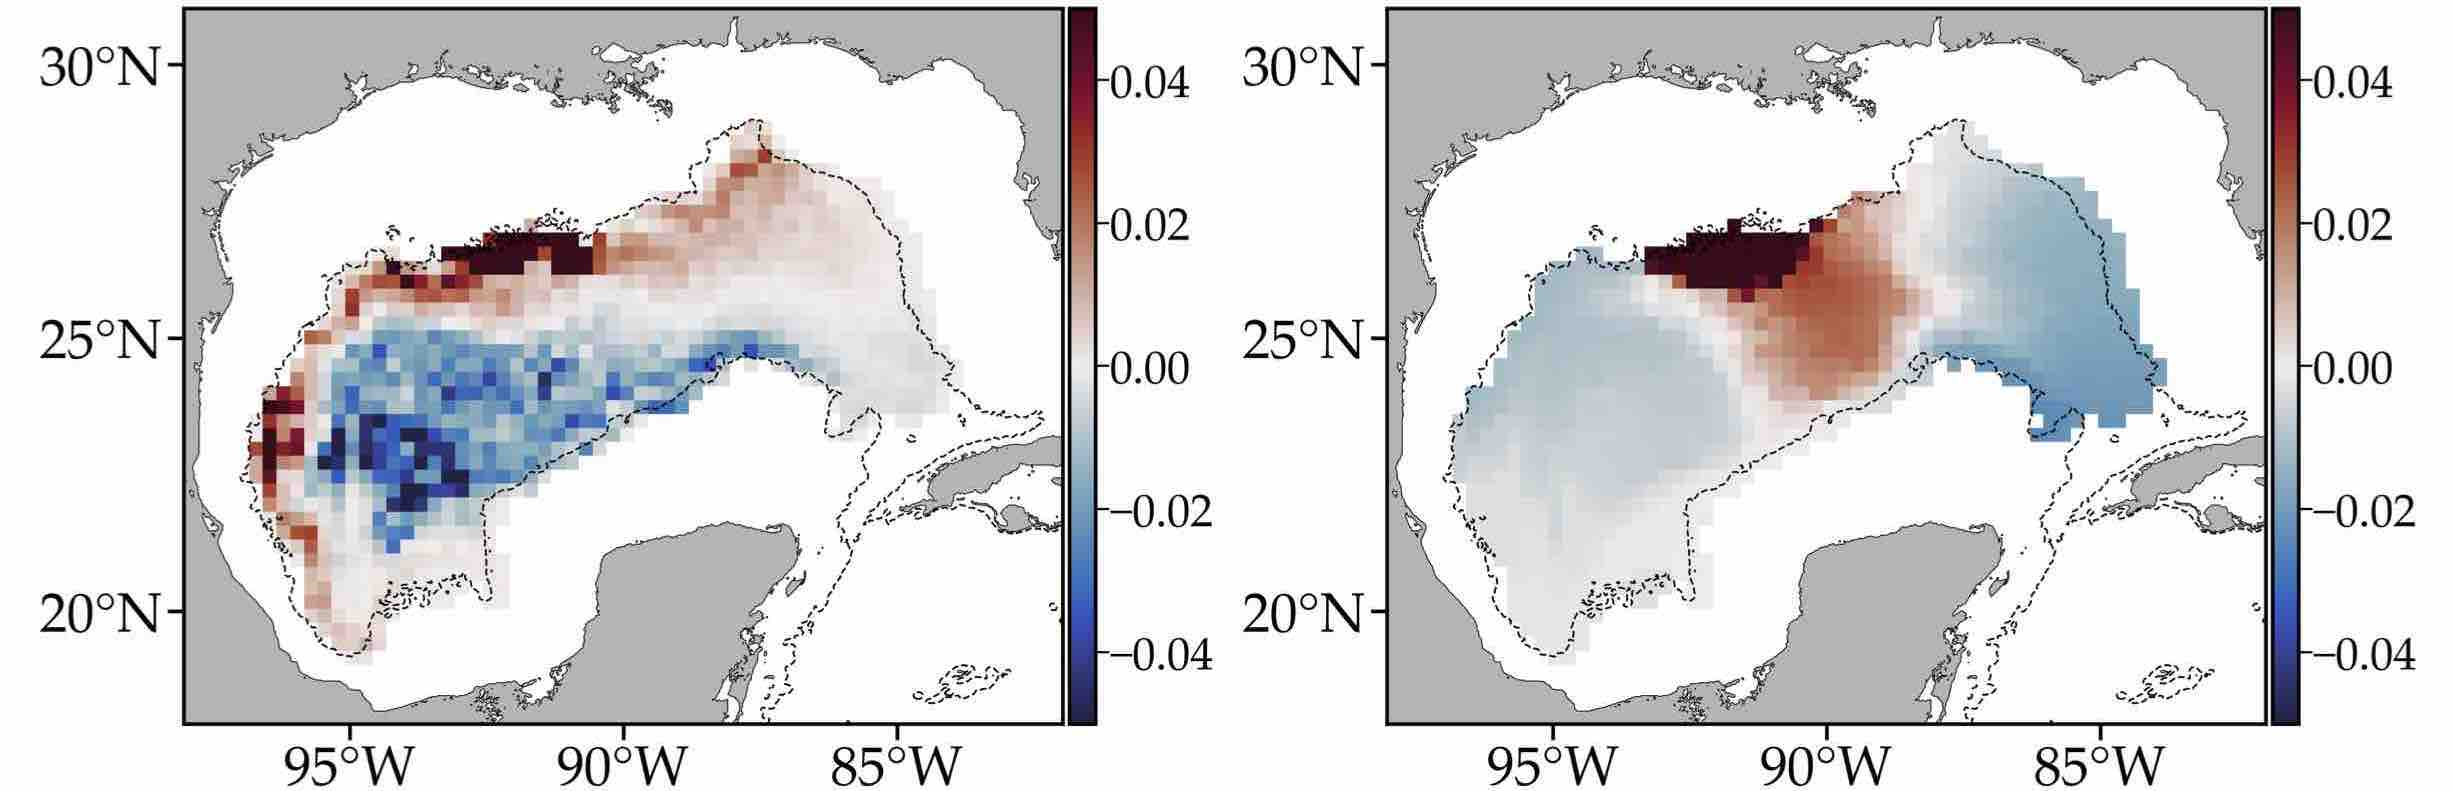
\includegraphics[width=\textwidth]{geogomdeep-fig08b.jpg}
\end{figure}
\begin{figure}
  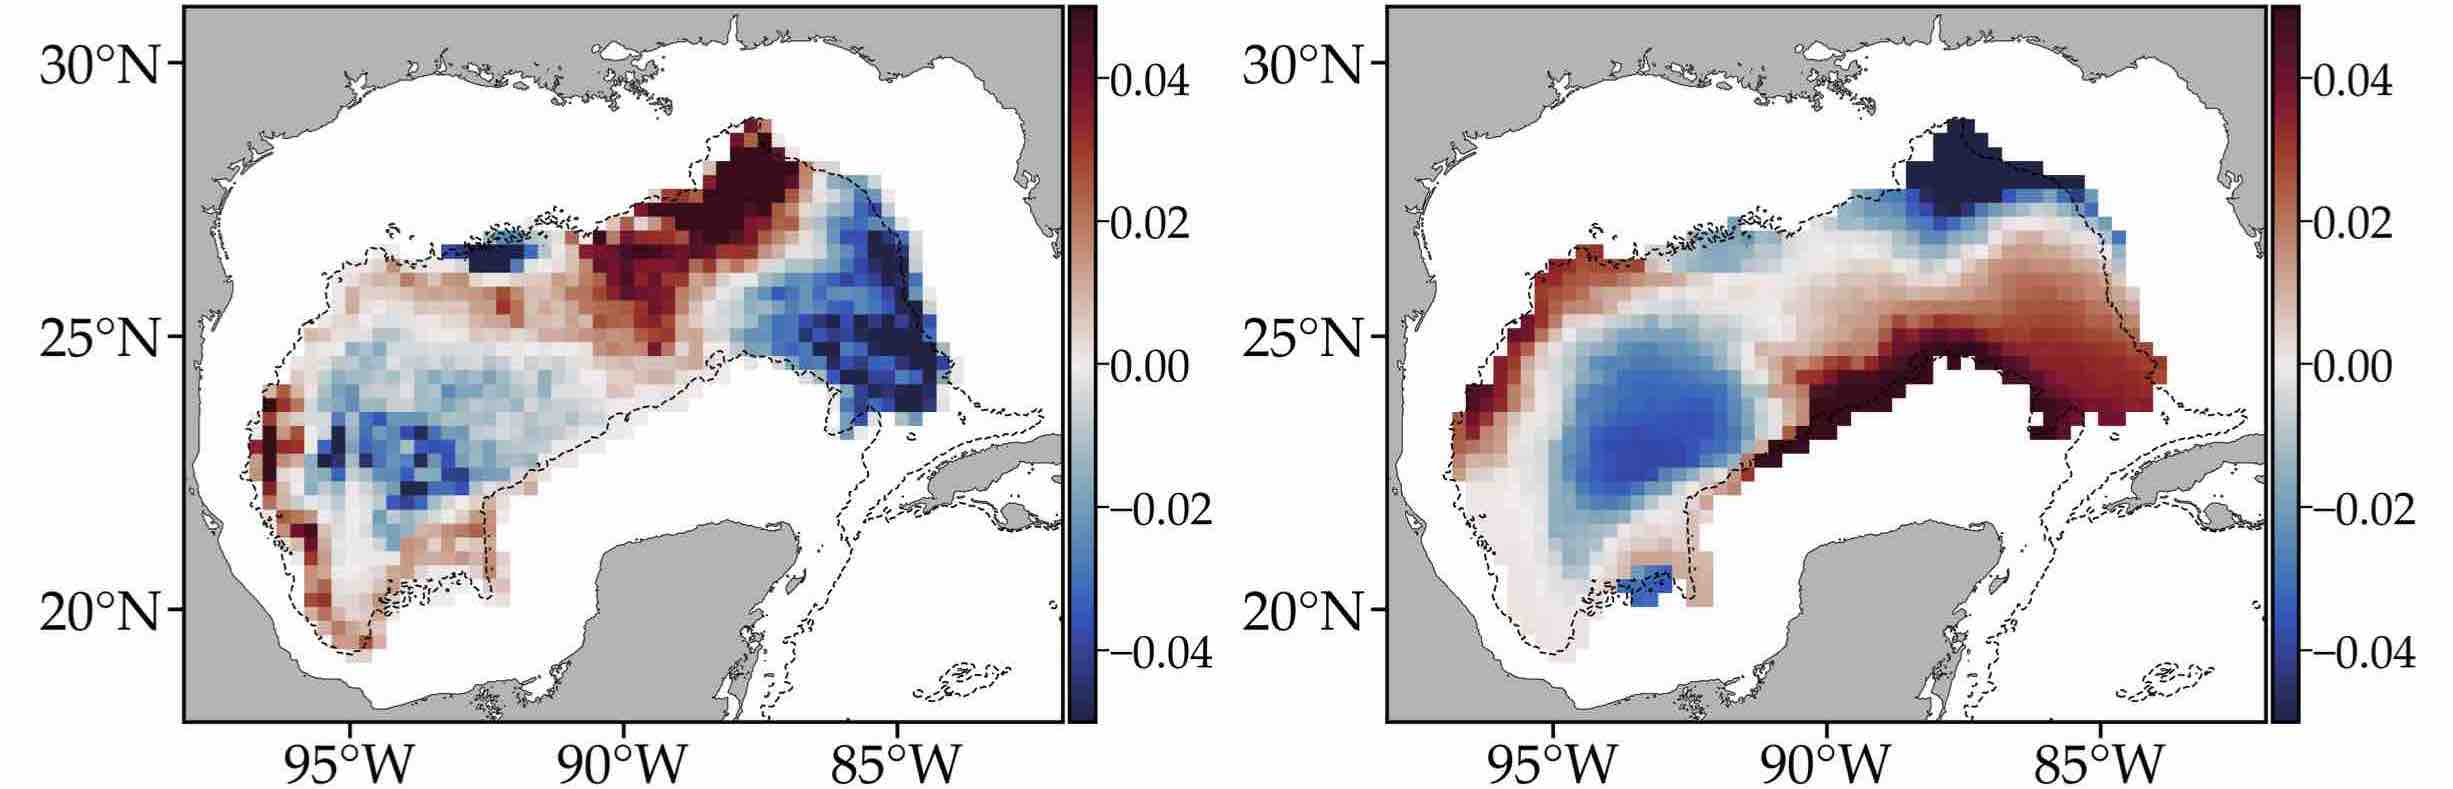
\includegraphics[width=\textwidth]{geogomdeep-fig08c.jpg}
\end{figure}
}
}

\frame{\frametitle{Lagrangian geography of the deep Gulf of Mexico}

Combination of the basins of attraction from the top right eigenvectors (by thresholding).
\begin{figure}
  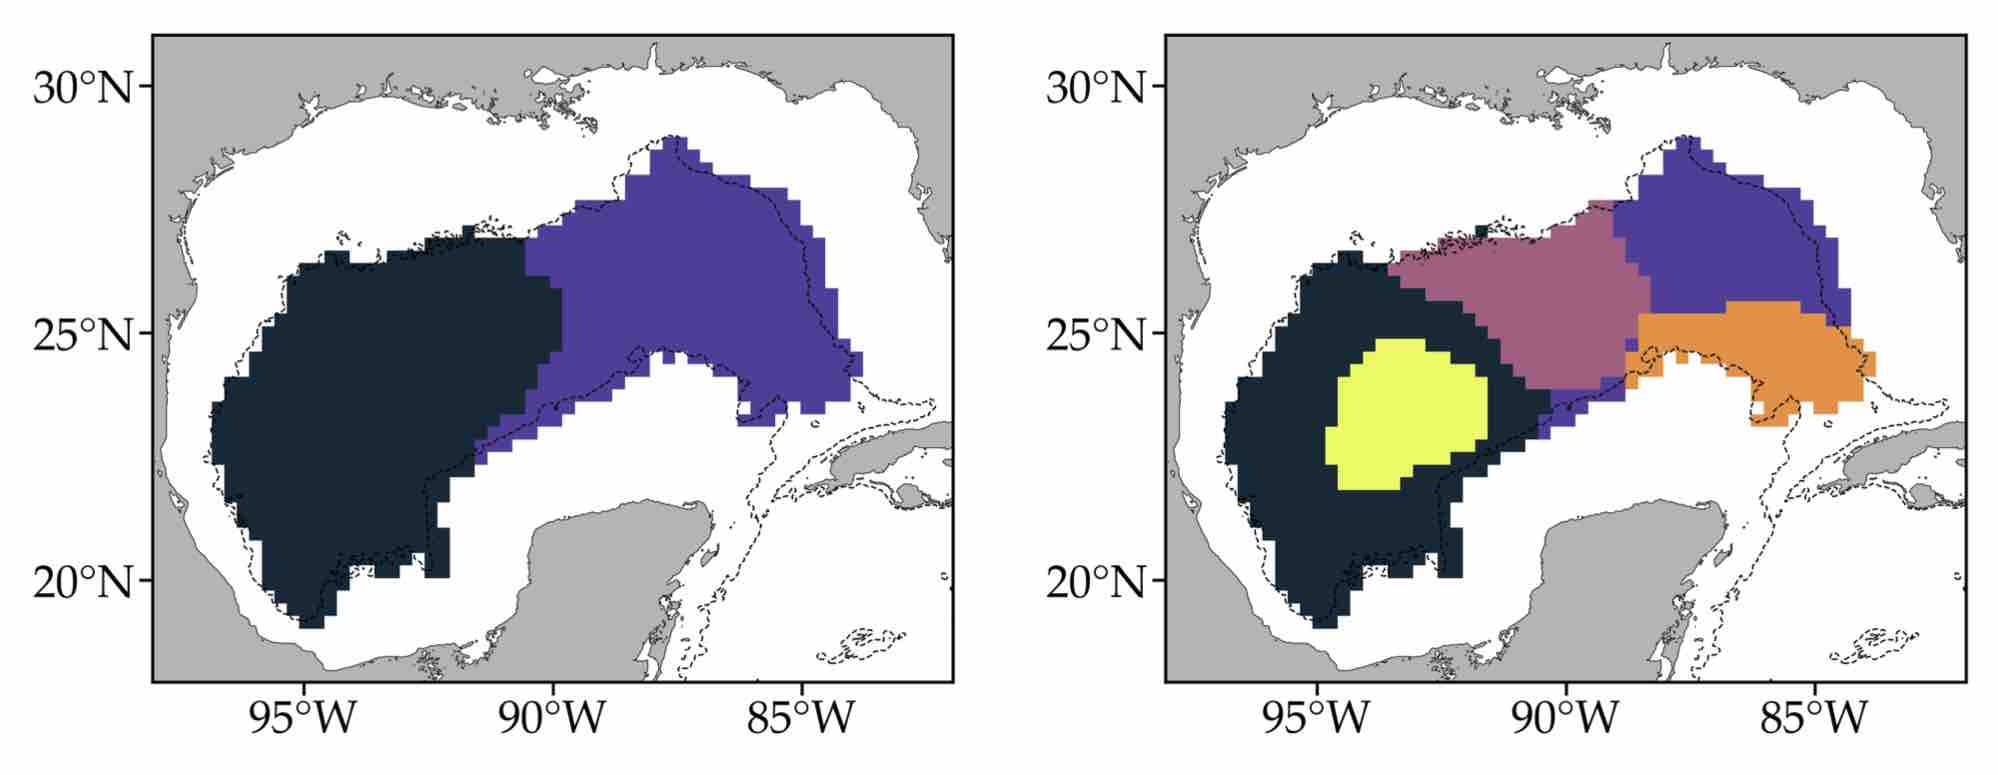
\includegraphics[width=0.9\textwidth]{geogomdeep-fig09.jpg}
\end{figure}

\begin{figure}
  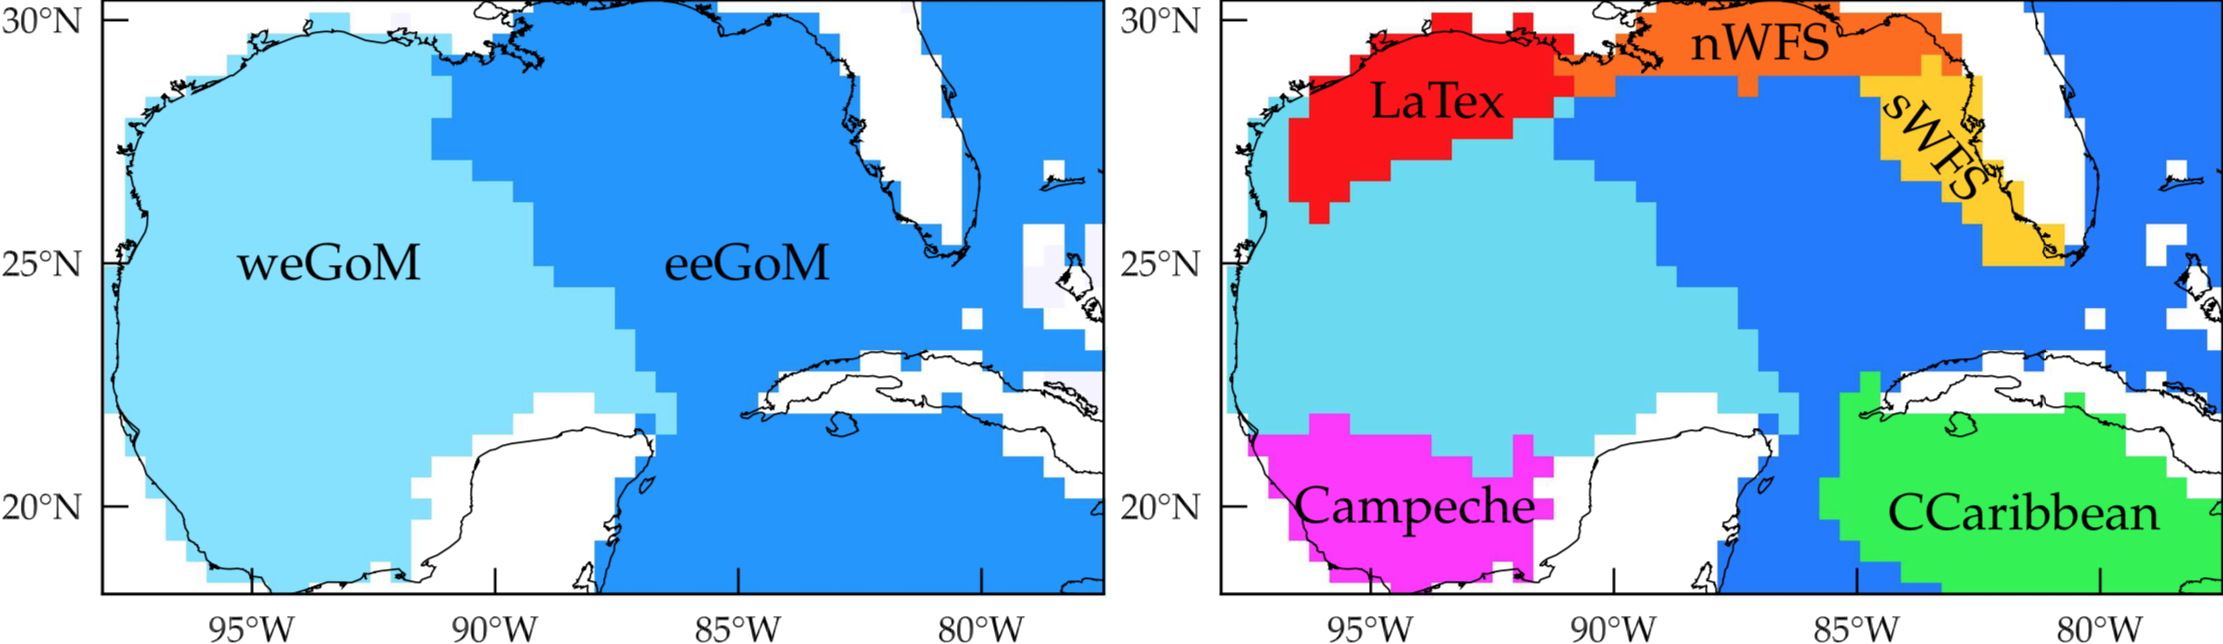
\includegraphics[width=0.9\textwidth]{geosurf.png}
\end{figure}
}

\frame{
\begin{figure}
  \only<1>{
  \frametitle{Connectivity matrix (1 week)}
  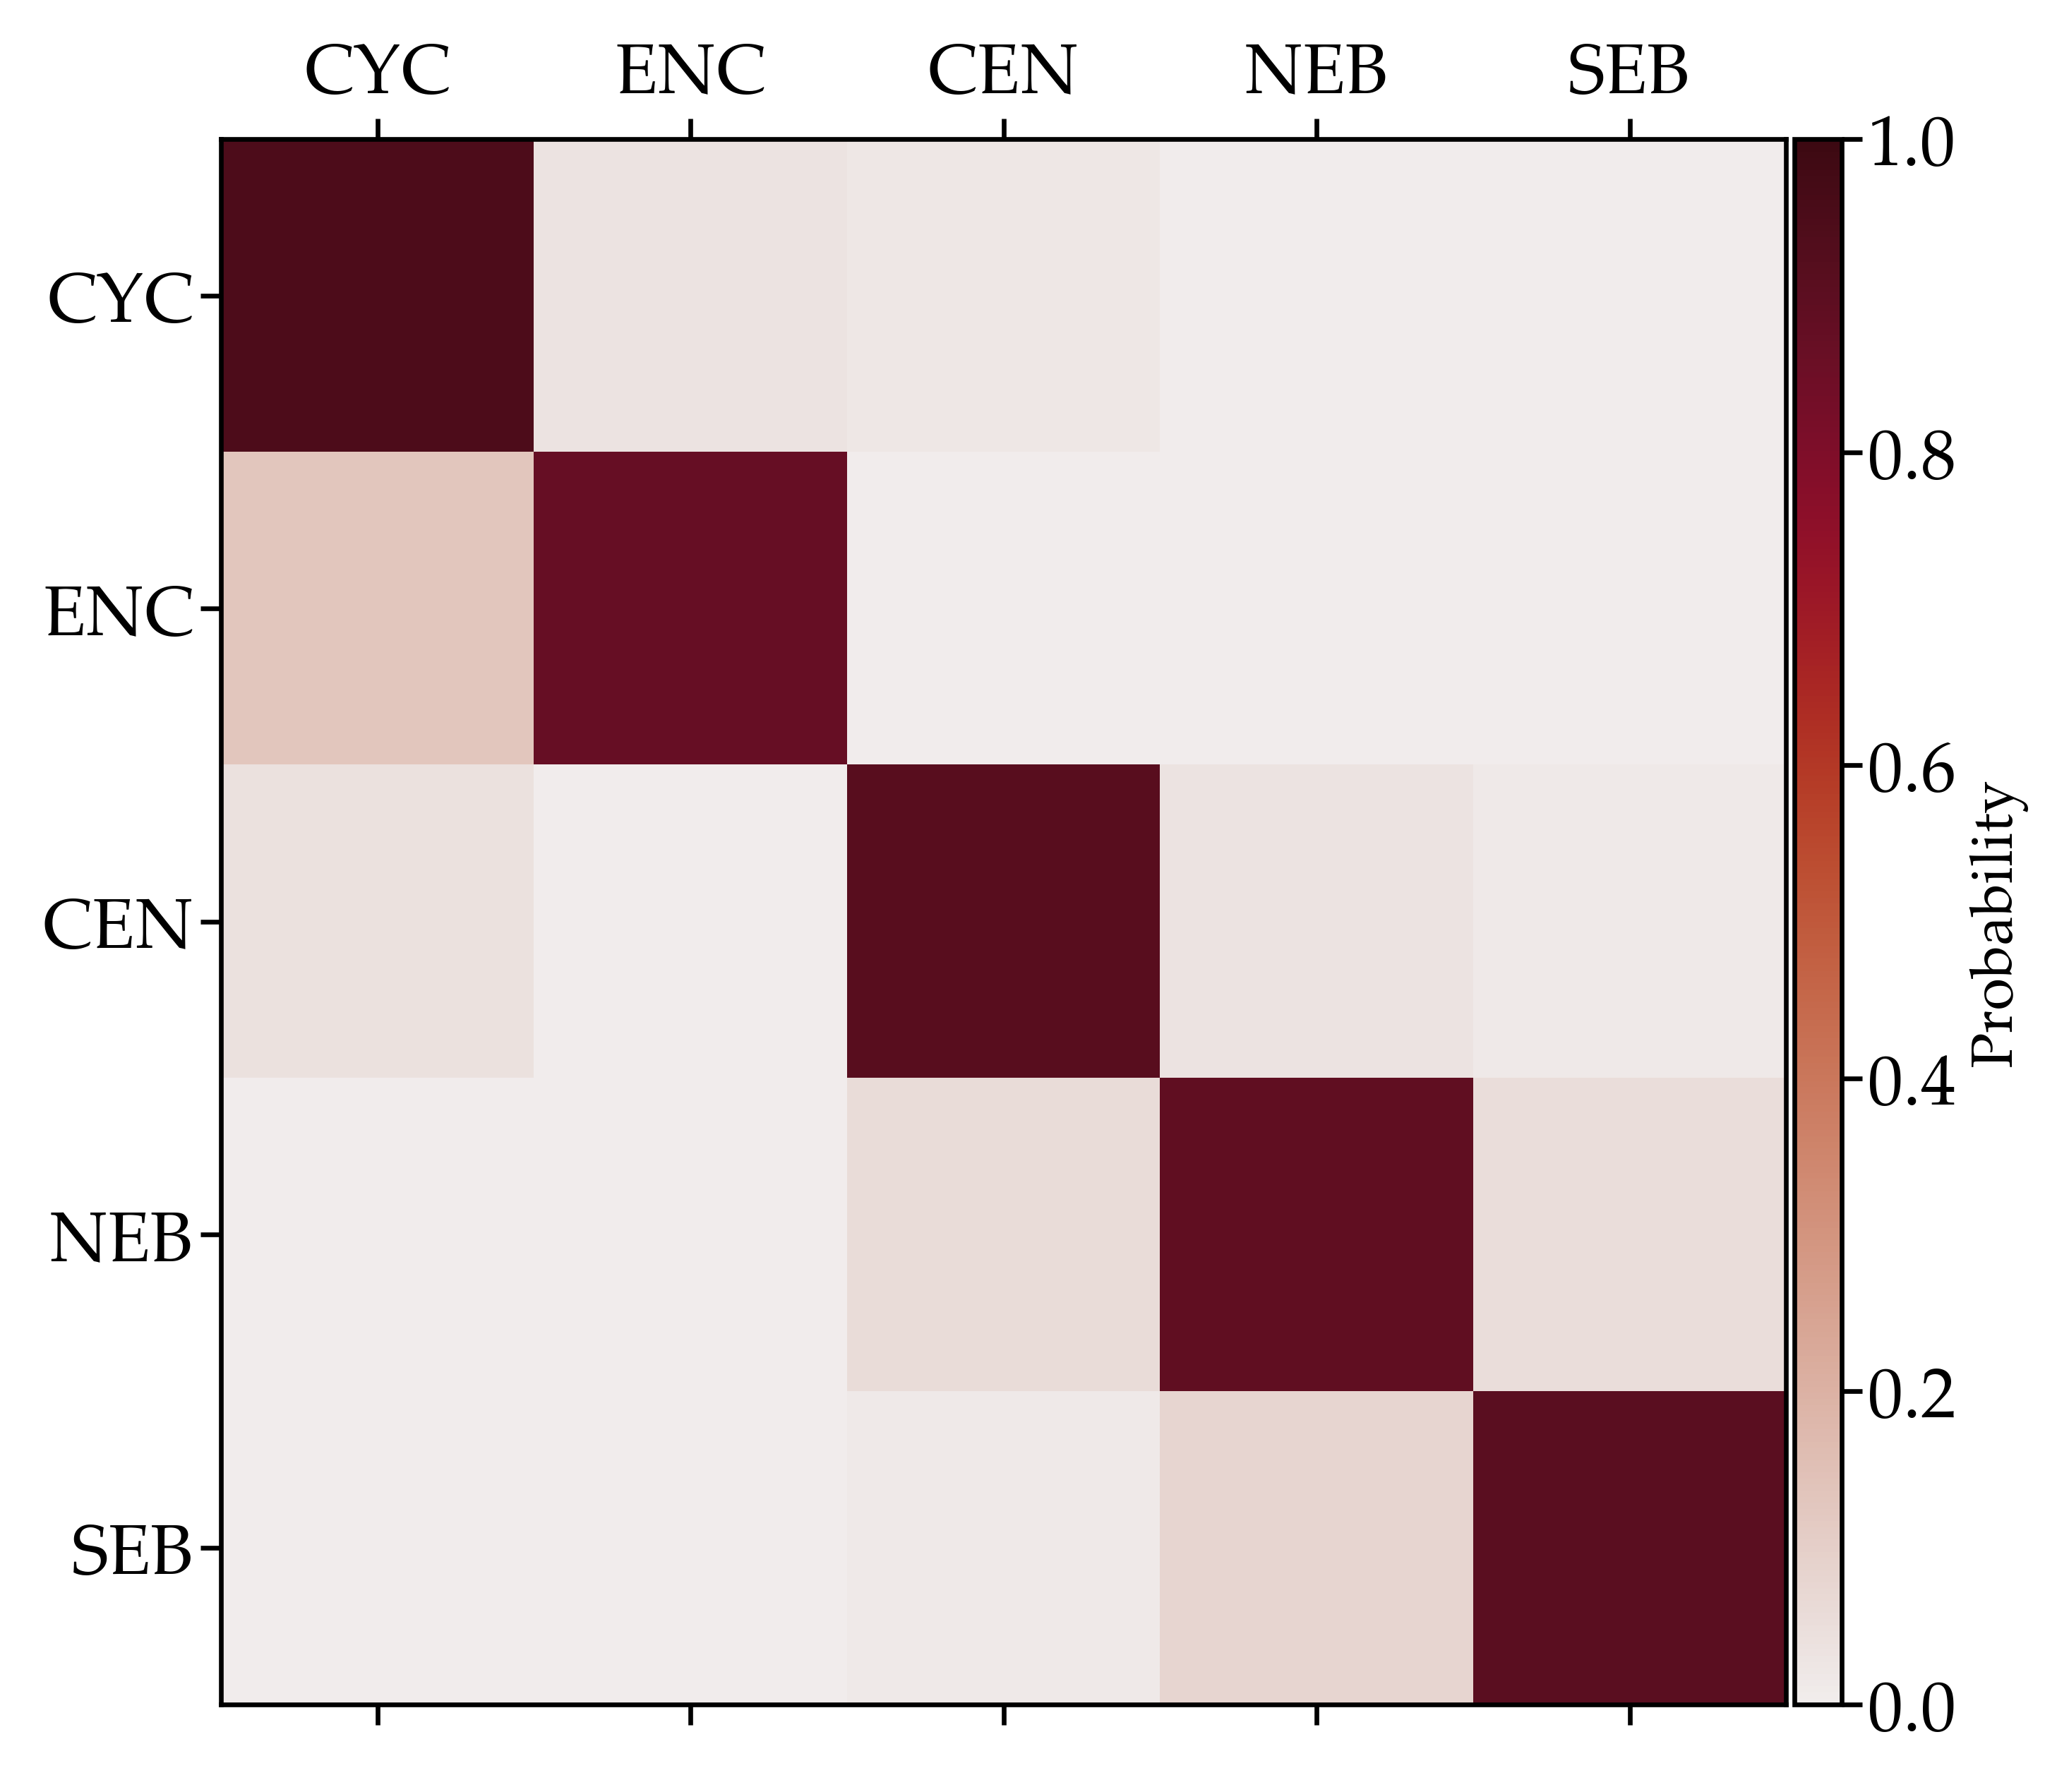
\includegraphics[width=0.9\textwidth]{1wconnection.png}
  }
  \only<2>{
  \frametitle{Connectivity matrix (2 weeks)}
  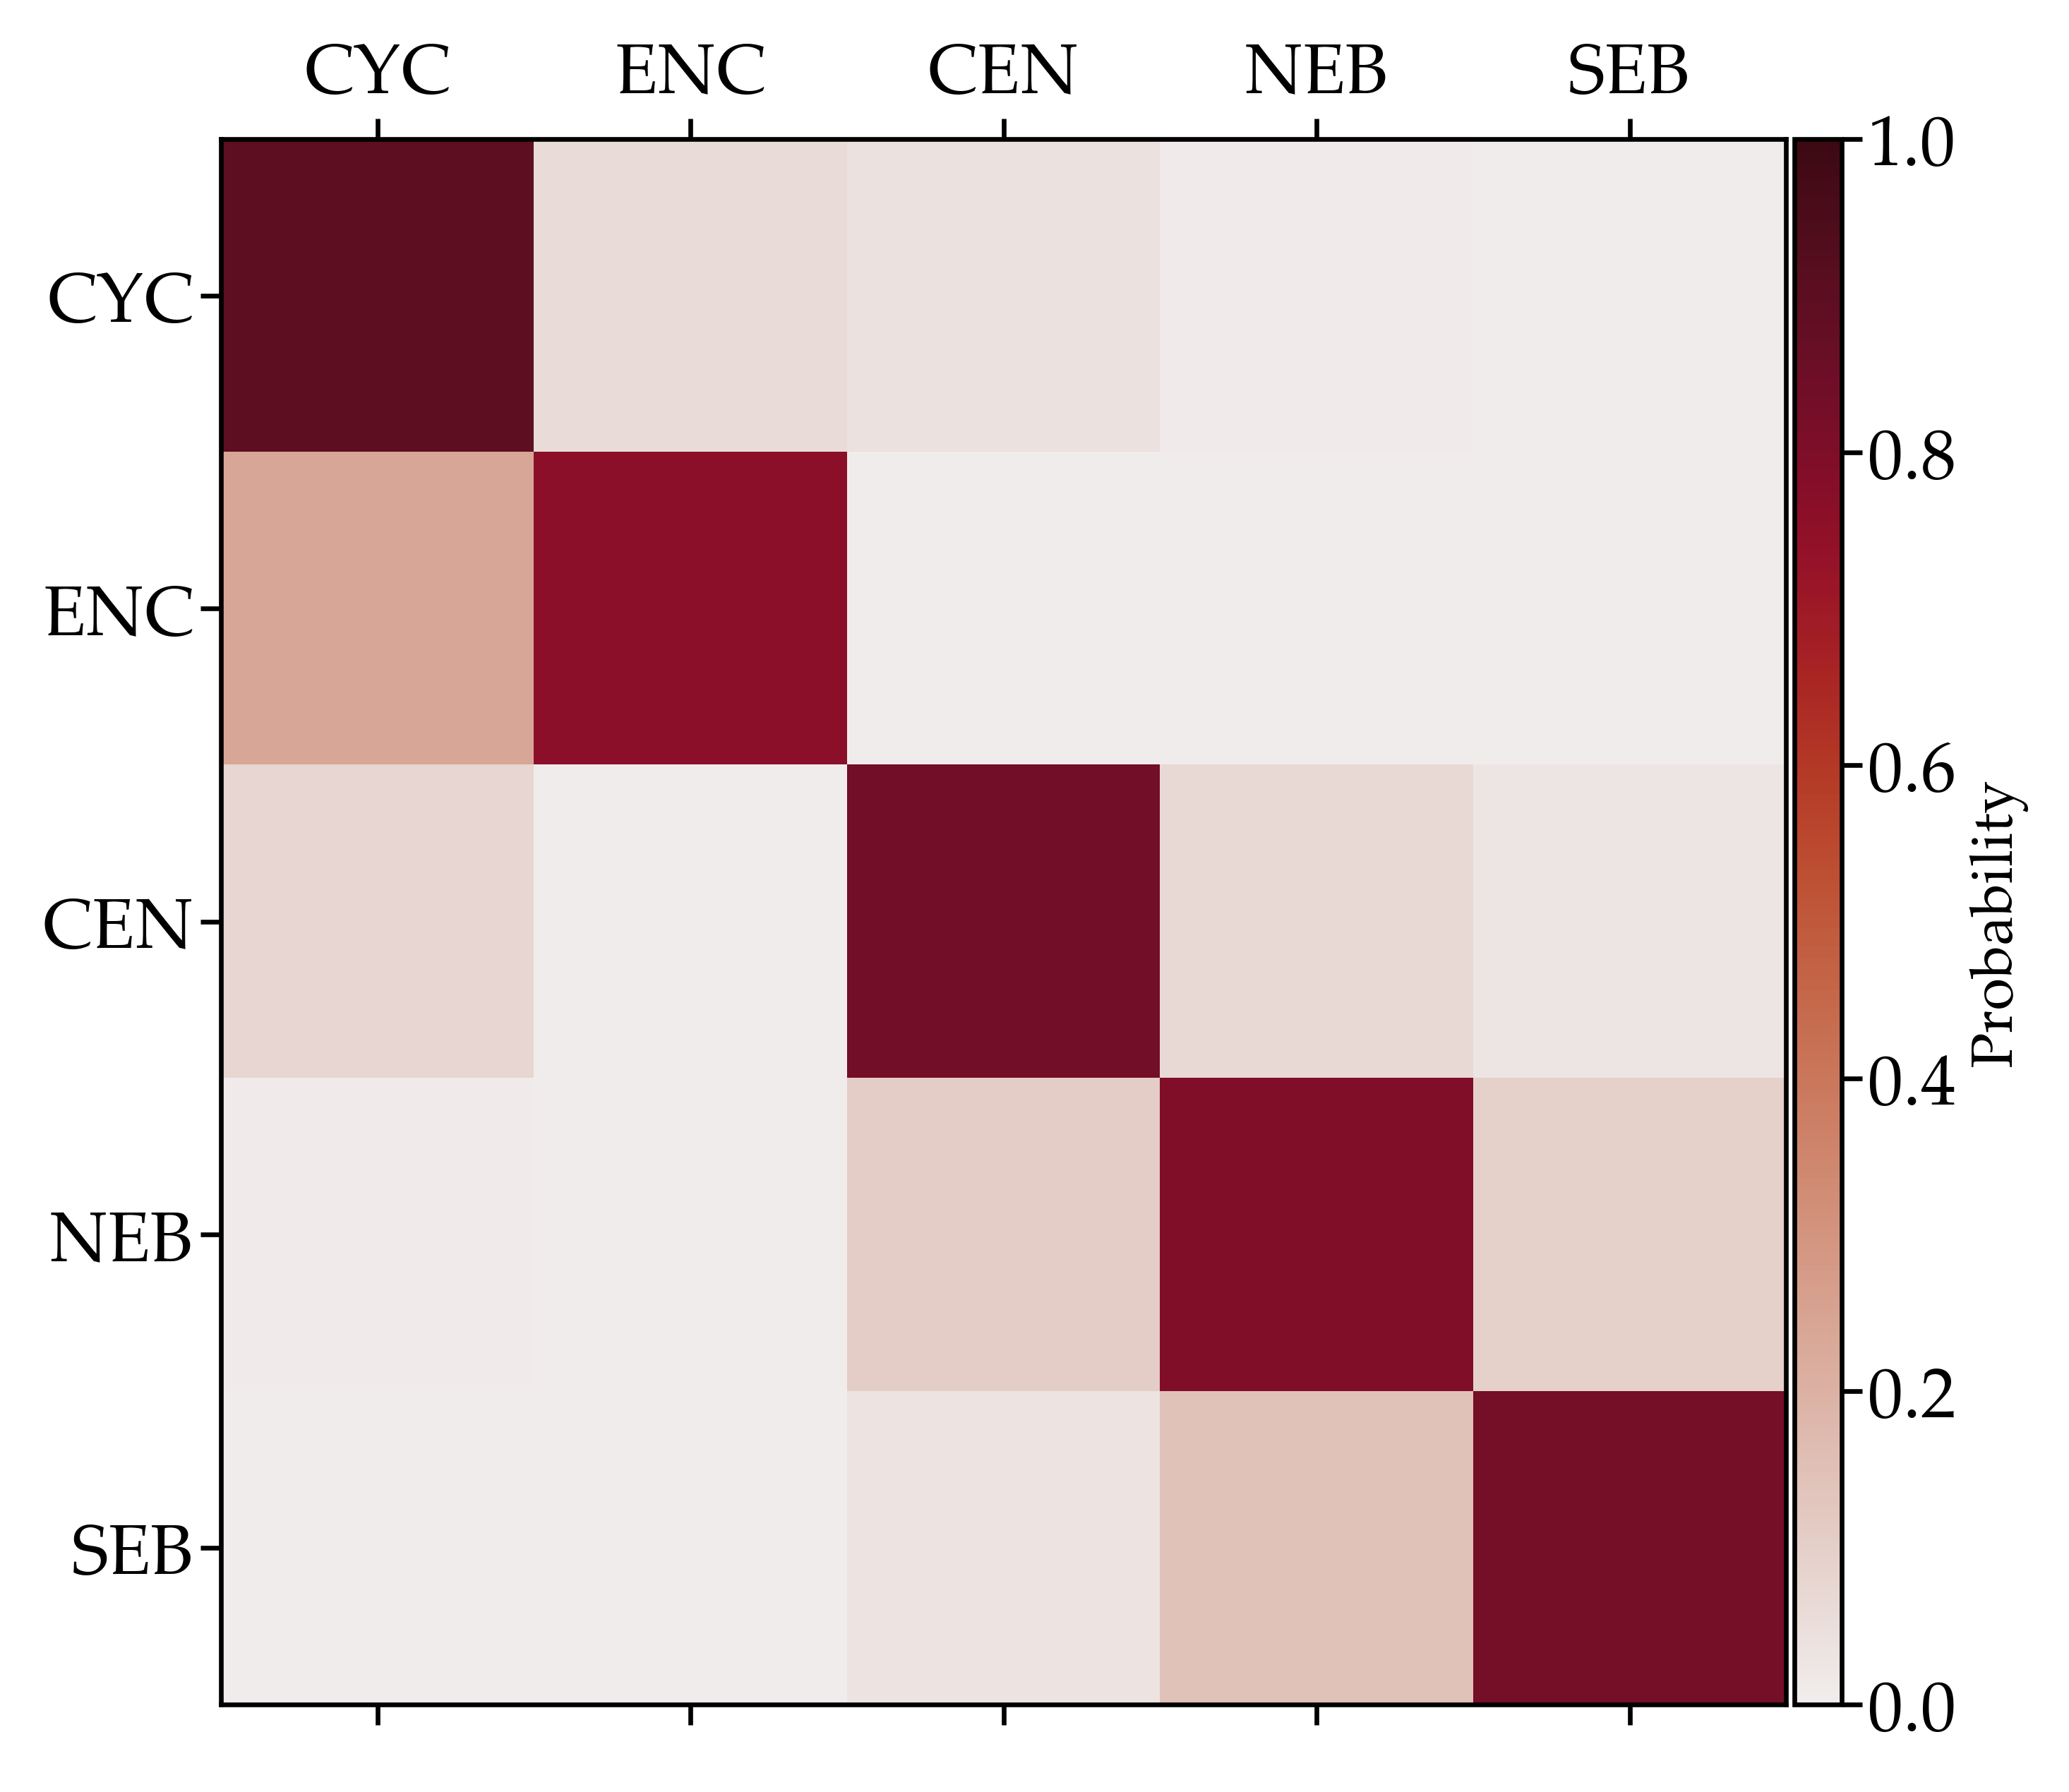
\includegraphics[width=0.9\textwidth]{2wconnection.png}
  }
  \only<3>{
  \frametitle{Connectivity matrix (4 weeks)}
  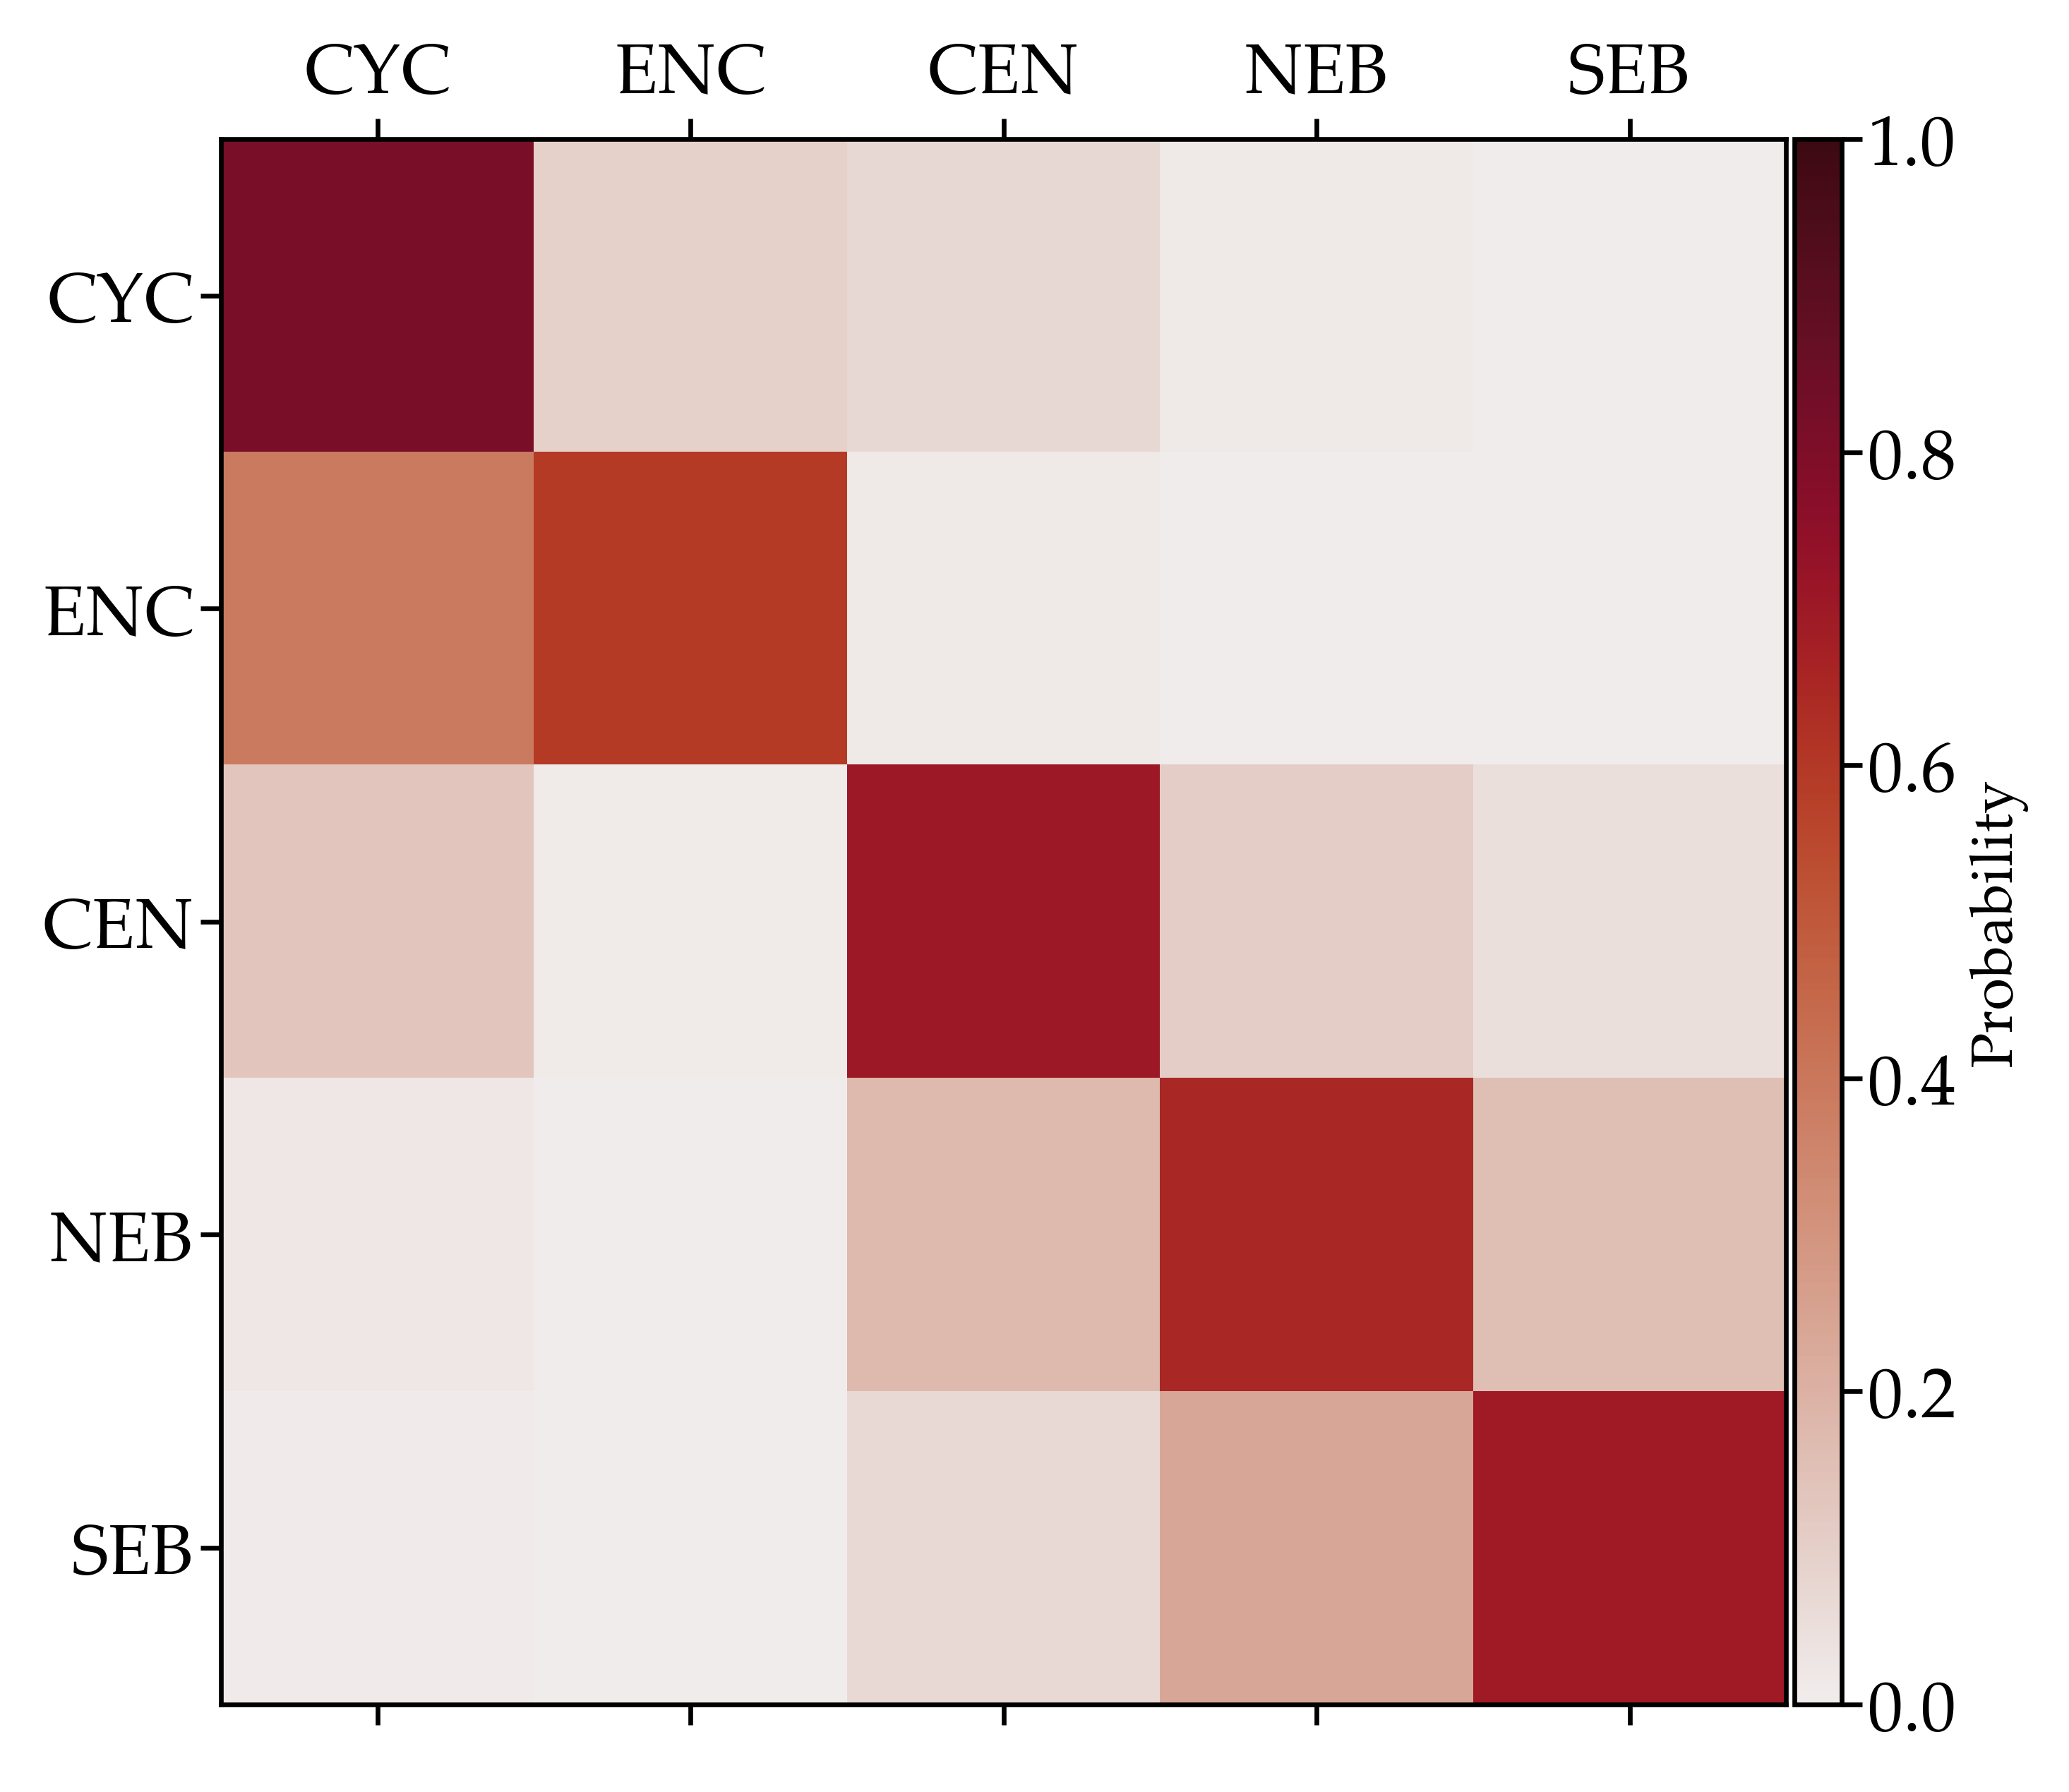
\includegraphics[width=0.9\textwidth]{4wconnection.png}
  }
\end{figure}
}


\frame{\frametitle{Residence time}
The time $\tau$ for a trajectory in box $B_i$ to move out of $A$, also known also as the mean time to hit the complement of $A$ \citep{Norris-98}.
\begin{equation} 
  (\Id - P|_A)\tau/T = \mathbf{1},
  \label{eq:tau}
\end{equation}
The time on average to reach a given province
starting from any province can be computed using \eqref{eq:tau} with $A$ set to the target province. We can see the cyclonic motion on the western region \citep{perez2017dominant}.
\begin{figure}
  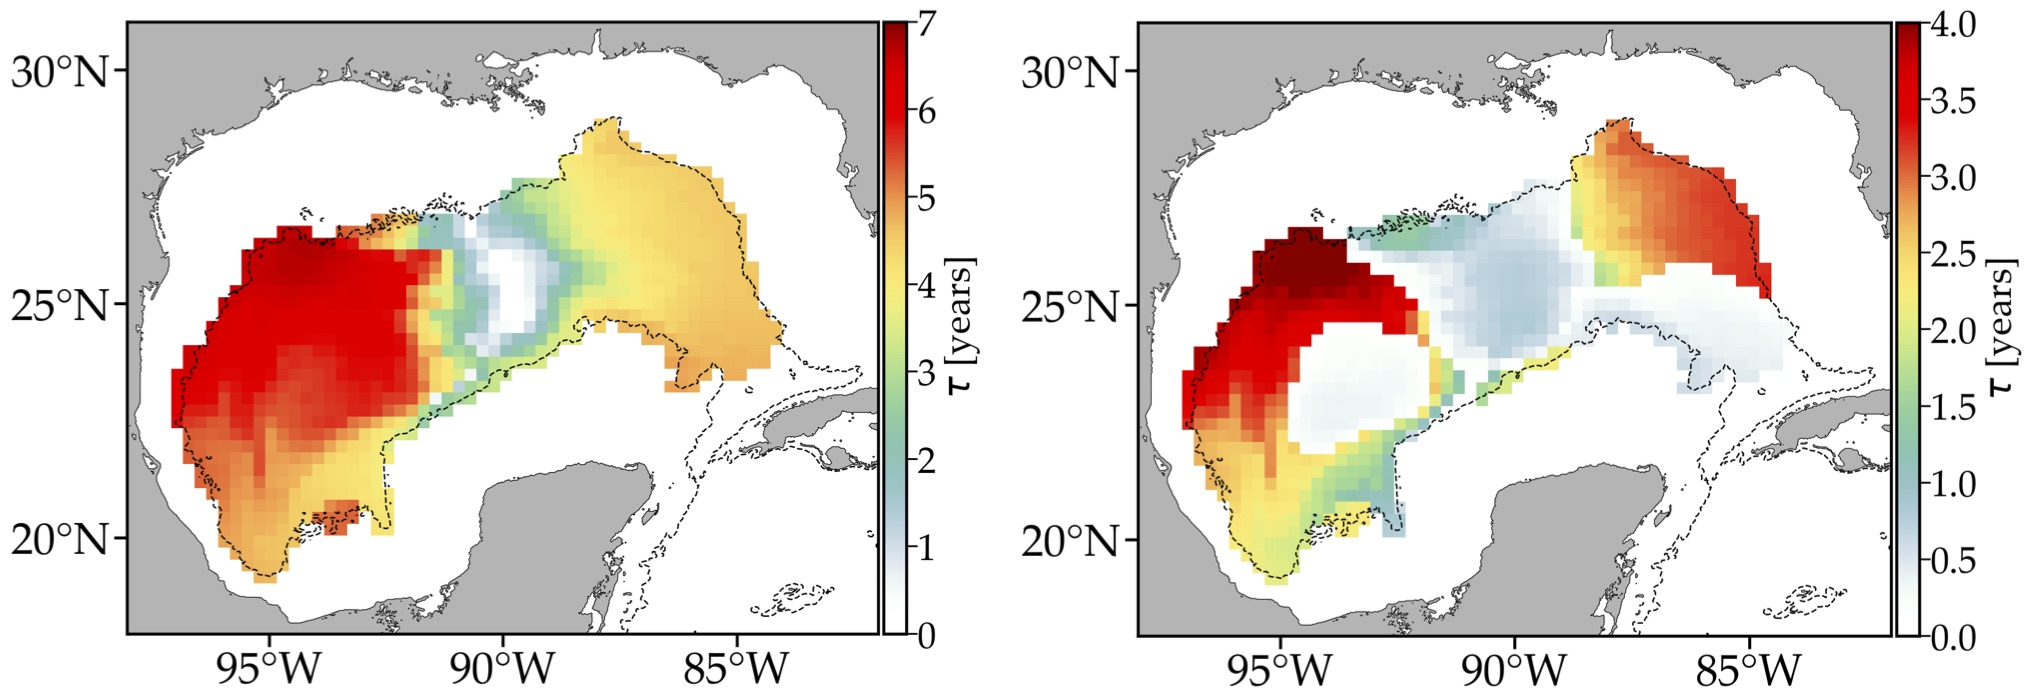
\includegraphics[width=\textwidth]{geogomdeep-figtau.jpg}
\end{figure}
}


\frame{\frametitle{Mean expected hitting time (complement of A in \eqref{eq:tau})}
\begin{figure}
    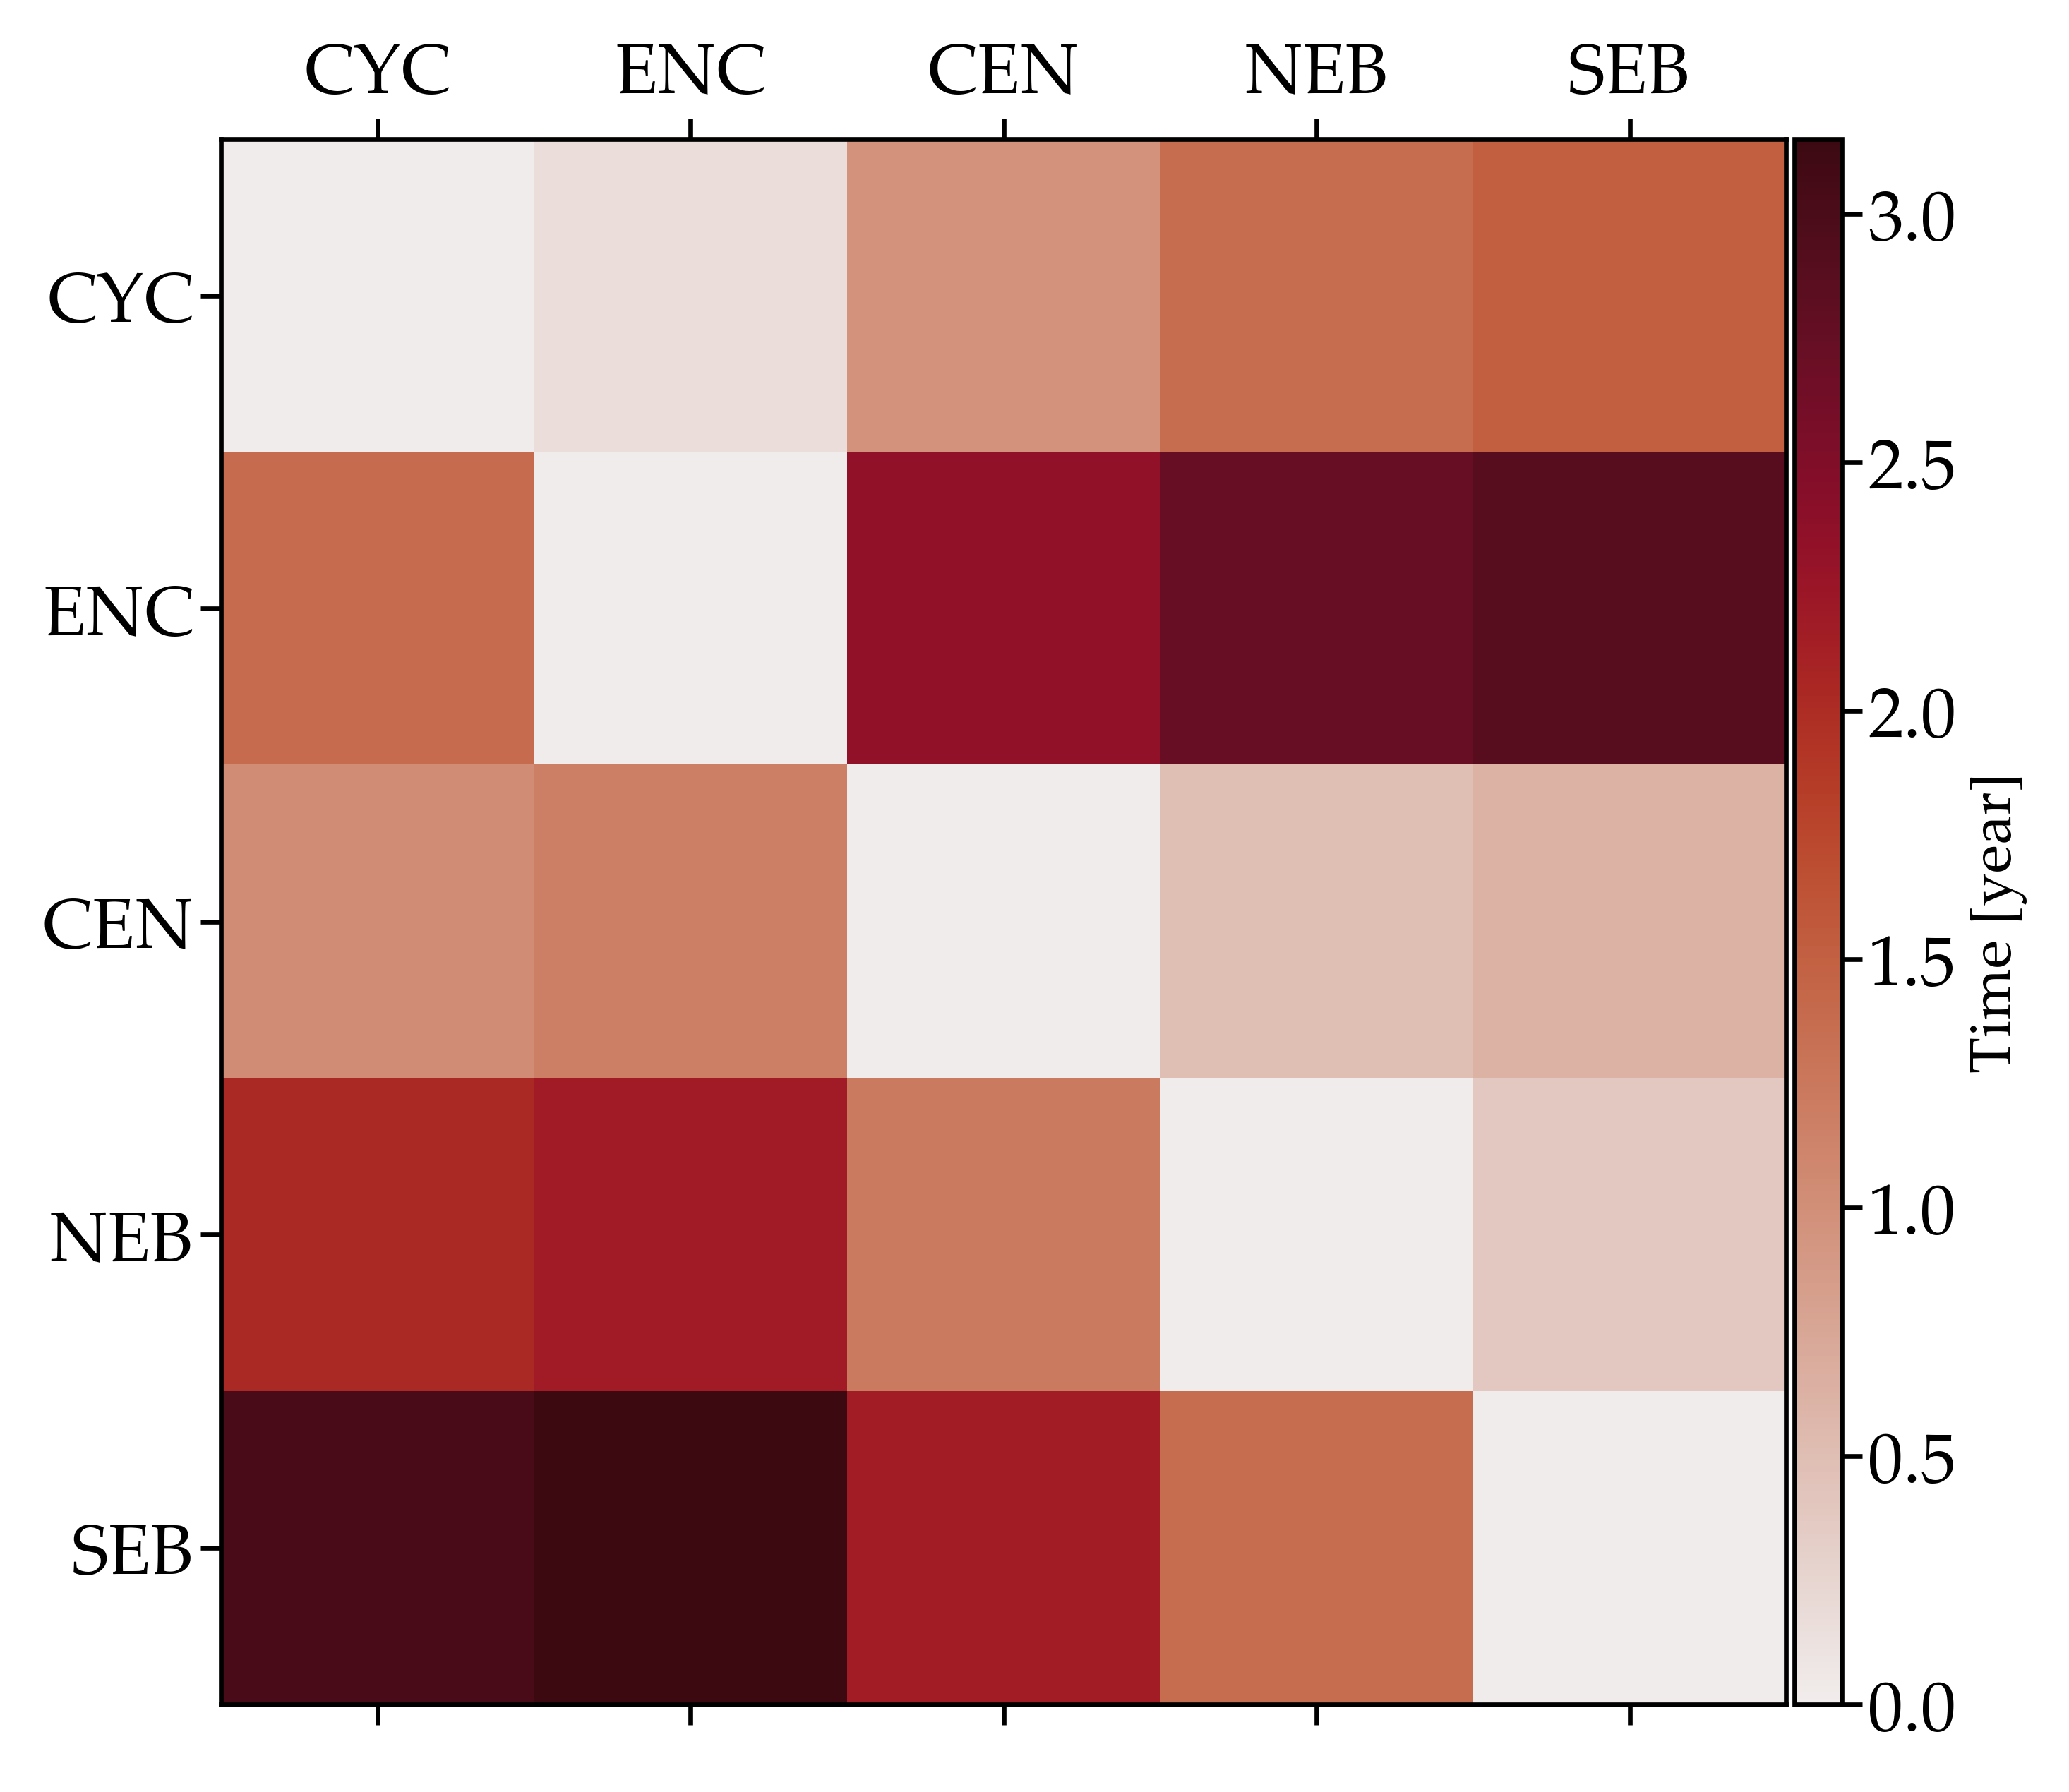
\includegraphics[width=0.9\textwidth]{hitting_time.png}
\end{figure}
}

\iffalse
\frame{\frametitle{Upwelling and Downwelling}
From incompressibility, accumulation can be used to approximate vertical velocity:
\begin{equation}
    a_i^{(k)} = \sum_j^N a_j (P^k)_{ji} \quad H_i^{(k)} = H \frac{a_i}{a_i^{(k)}} \quad w \sim \frac{H_i^{(k)} - H}{k T}
\end{equation}

\begin{figure}
  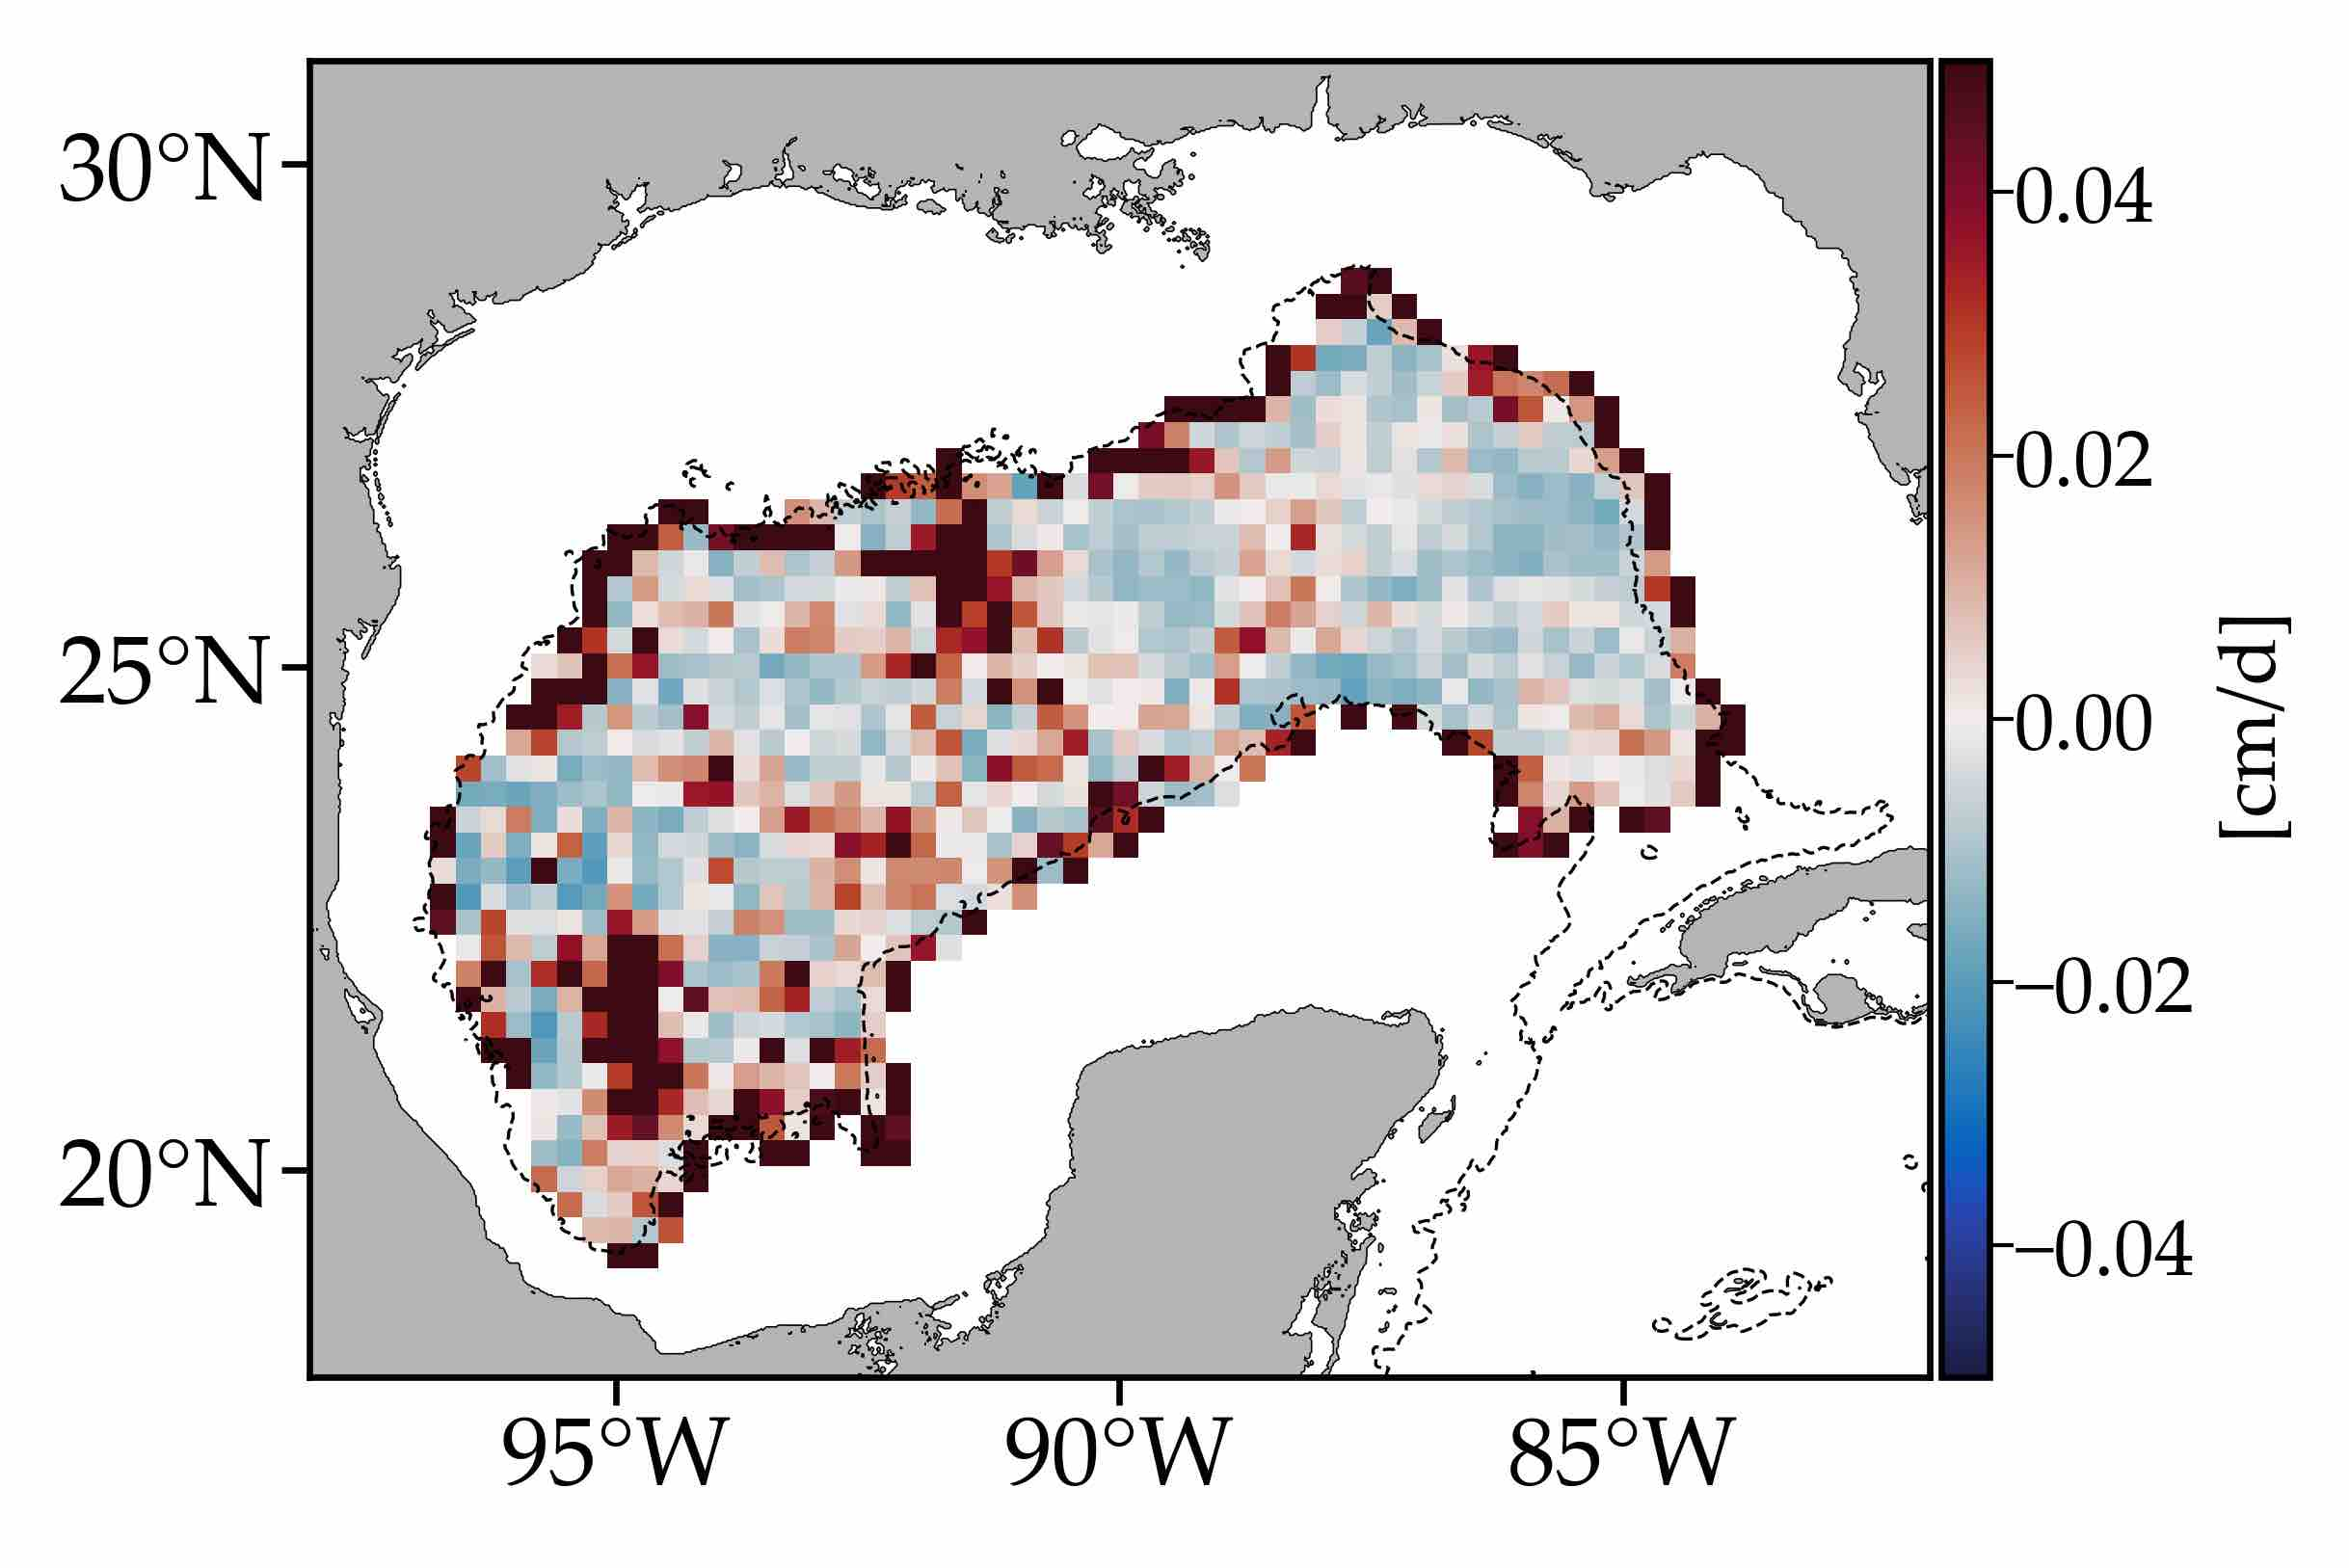
\includegraphics[width=8.5cm]{geogomdeep-fig05.jpg}
\end{figure}
}
\fi

\frame{\frametitle{Validation with experimental data \citep{ledwell2016dispersion}}
Tracer mostly spreads along the continental slope and across Eastern bassin.
\begin{figure}
  \centering
  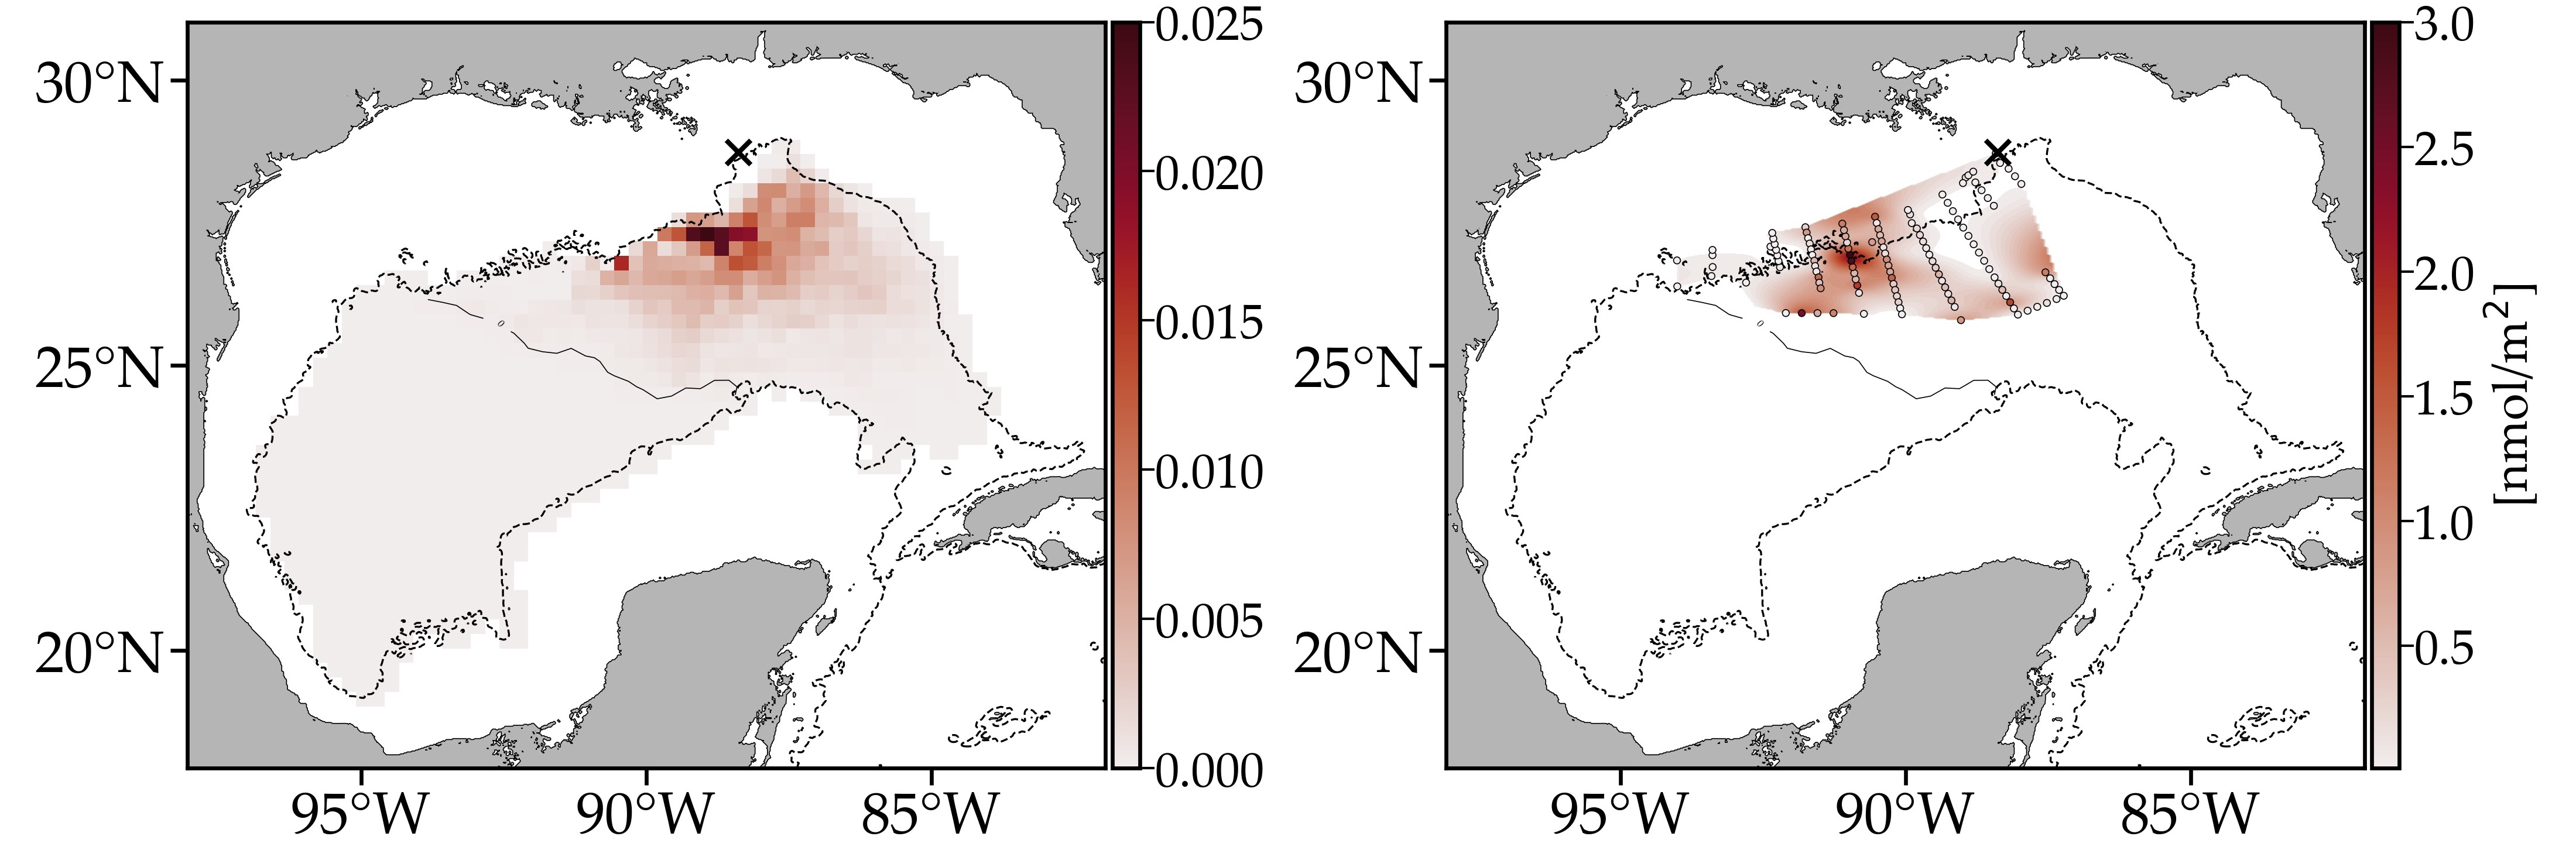
\includegraphics[width=1\textwidth]{geogomdeep-fig11.jpg}
  
  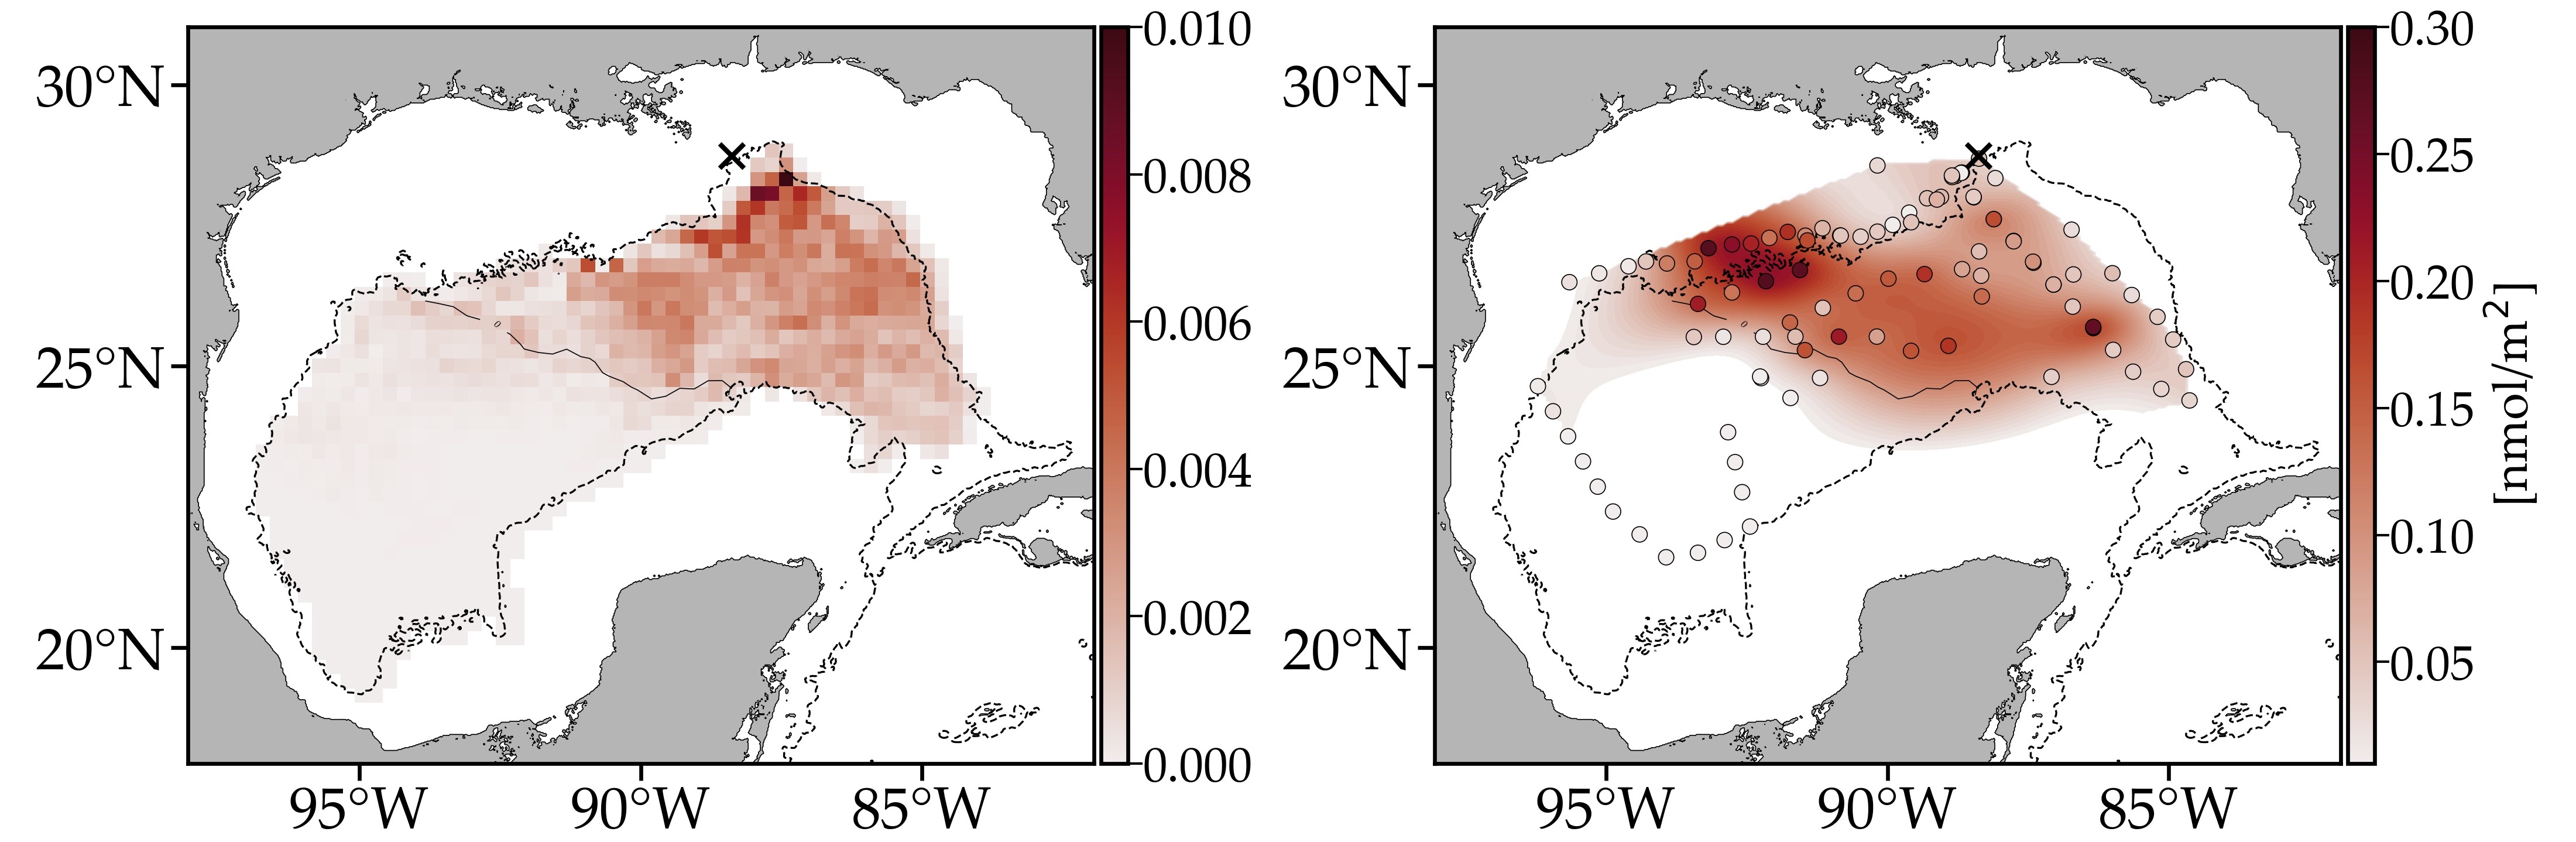
\includegraphics[width=1\textwidth]{geogomdeep-fig11b.jpg}
\end{figure}
}

\section{Conclusion}
\frame{\frametitle{Conclusion}

\begin{itemize}
	\item Assuming 3-d volume conservation, vertical flows over 1 yr is $\overline{w} = 0.2242$\, m/d
	\item Flow is mostly horizontal and ventilated from the Caribbean Sea (also explains why no float escape?)
	\item Fast spreading ($\approx 1$ yr over the eastern part) as observed by \cite{ledwell2016dispersion}
	\item Main partition is also reveal by the Argo floats
\end{itemize}

Future plans:
\begin{itemize}
	\item Evaluation of global circulation from surface drifters (GDP) and deep water floats (RAFOS, SOFAR \& ARGO)
\end{itemize}
}


\frame{\frametitle{Main partition from Argo floats}
\begin{figure}
  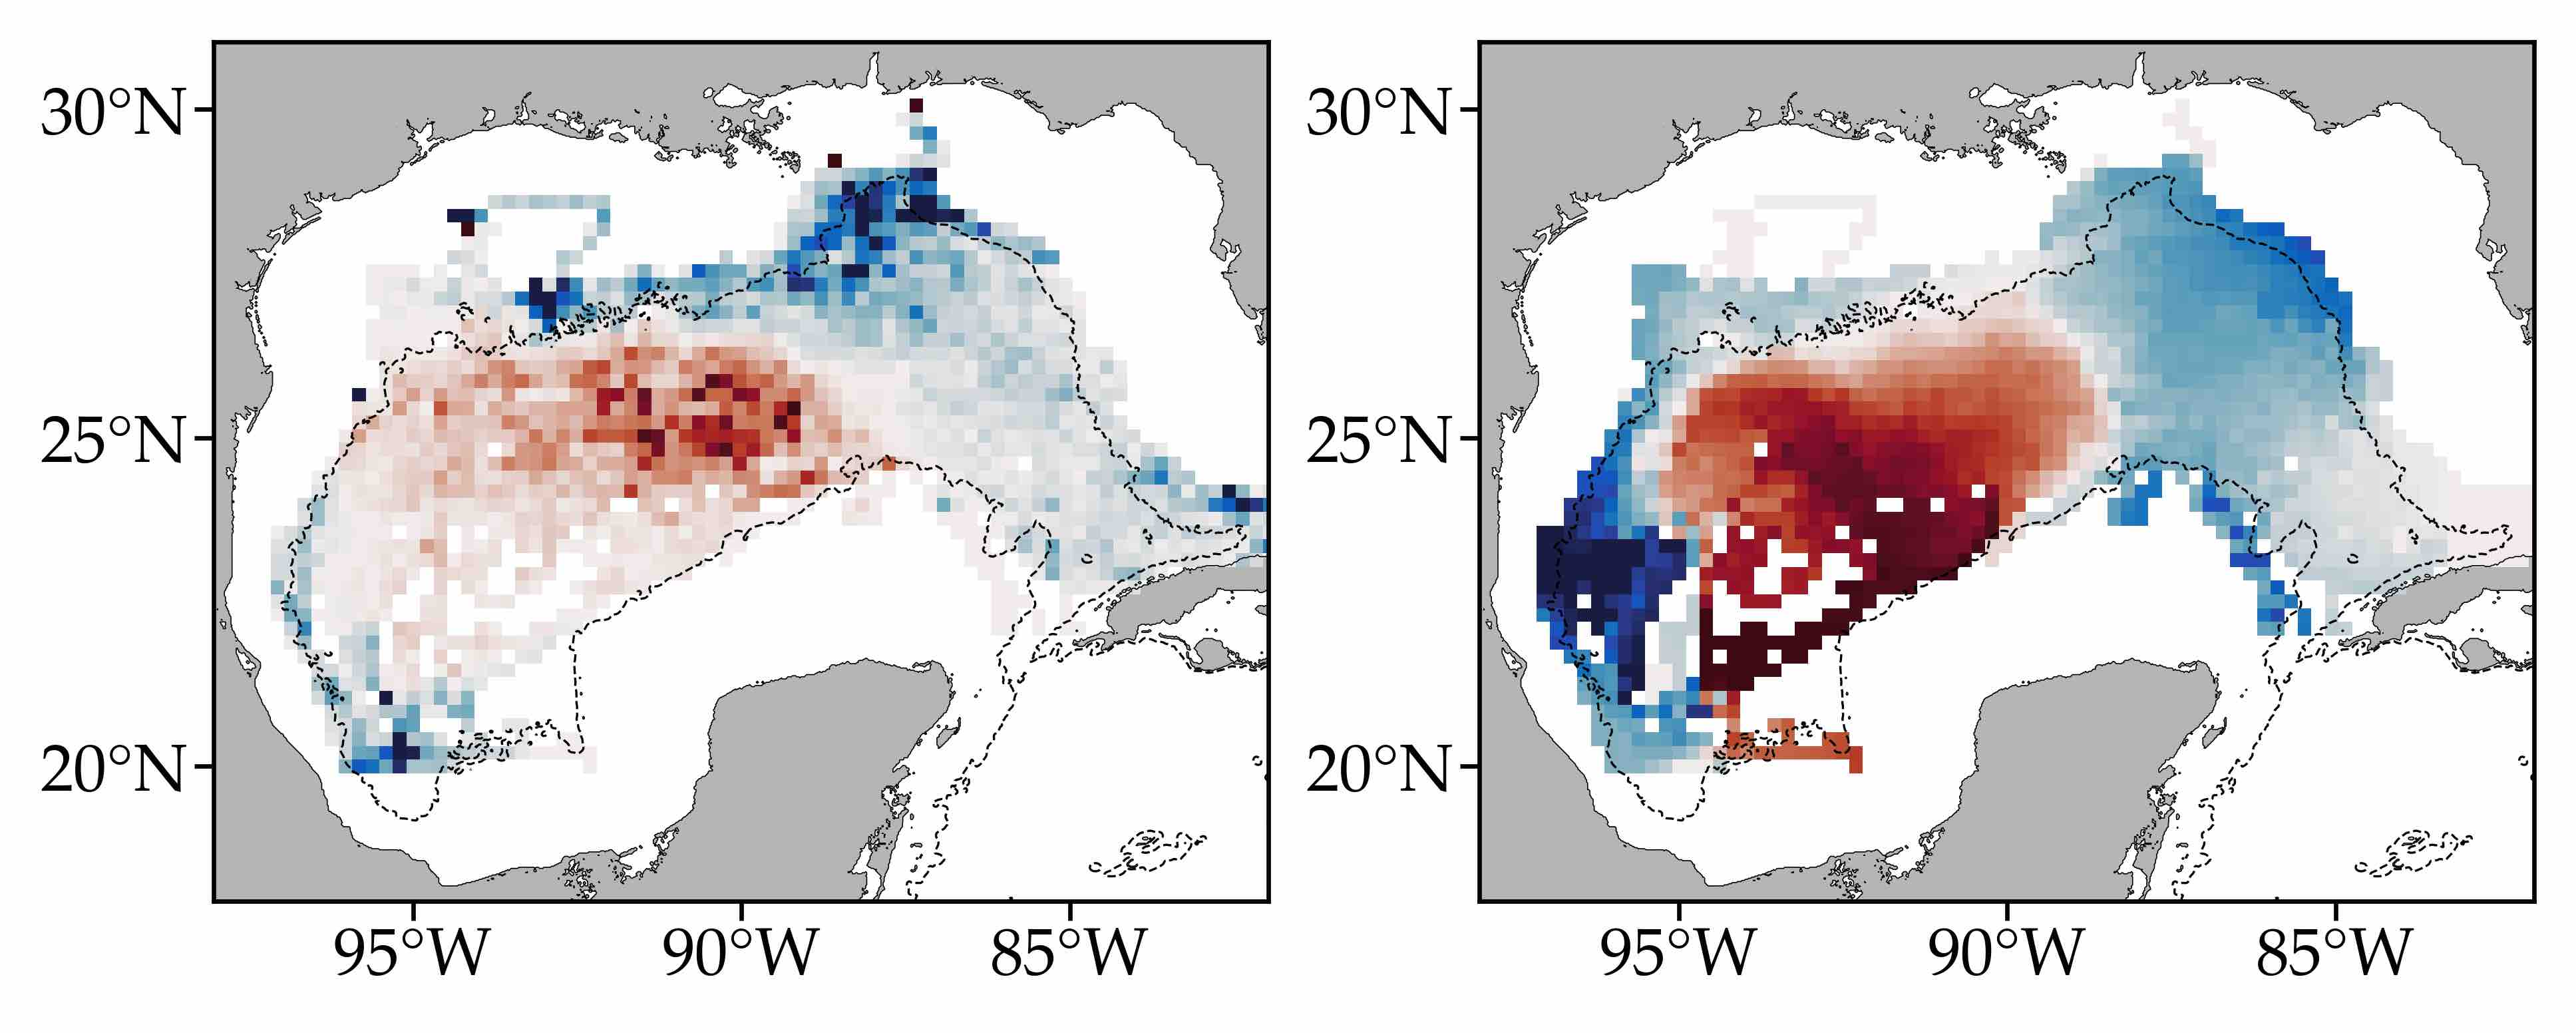
\includegraphics[width=\textwidth]{geogomdeep-fig12.jpg}
\end{figure}
}

\frame{\frametitle{Push forward in the Eastern corner of the domain}
\begin{figure}
  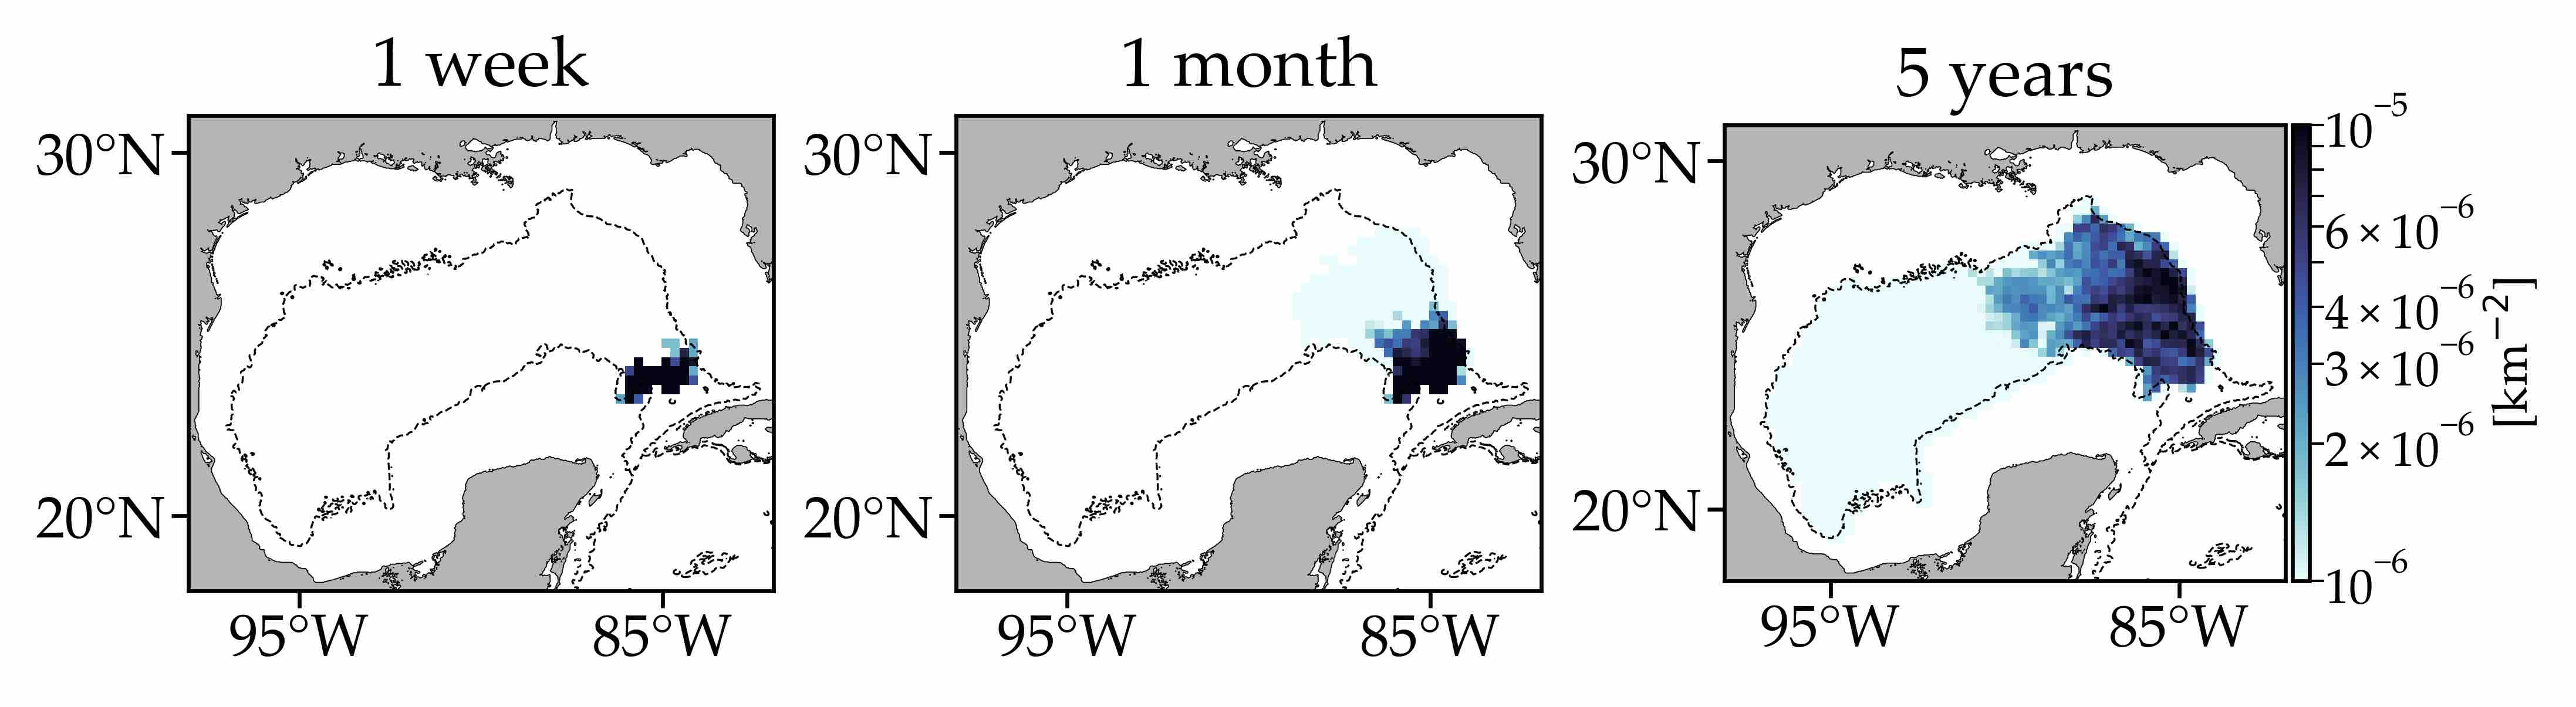
\includegraphics[width=\textwidth]{geogomdeep-fig14.jpg}
\end{figure}
}

\frame{\frametitle{Eigenvalues cut-off}
Look at the effect of random noise in the float trajectories on the eigenvalues.
\begin{figure}
  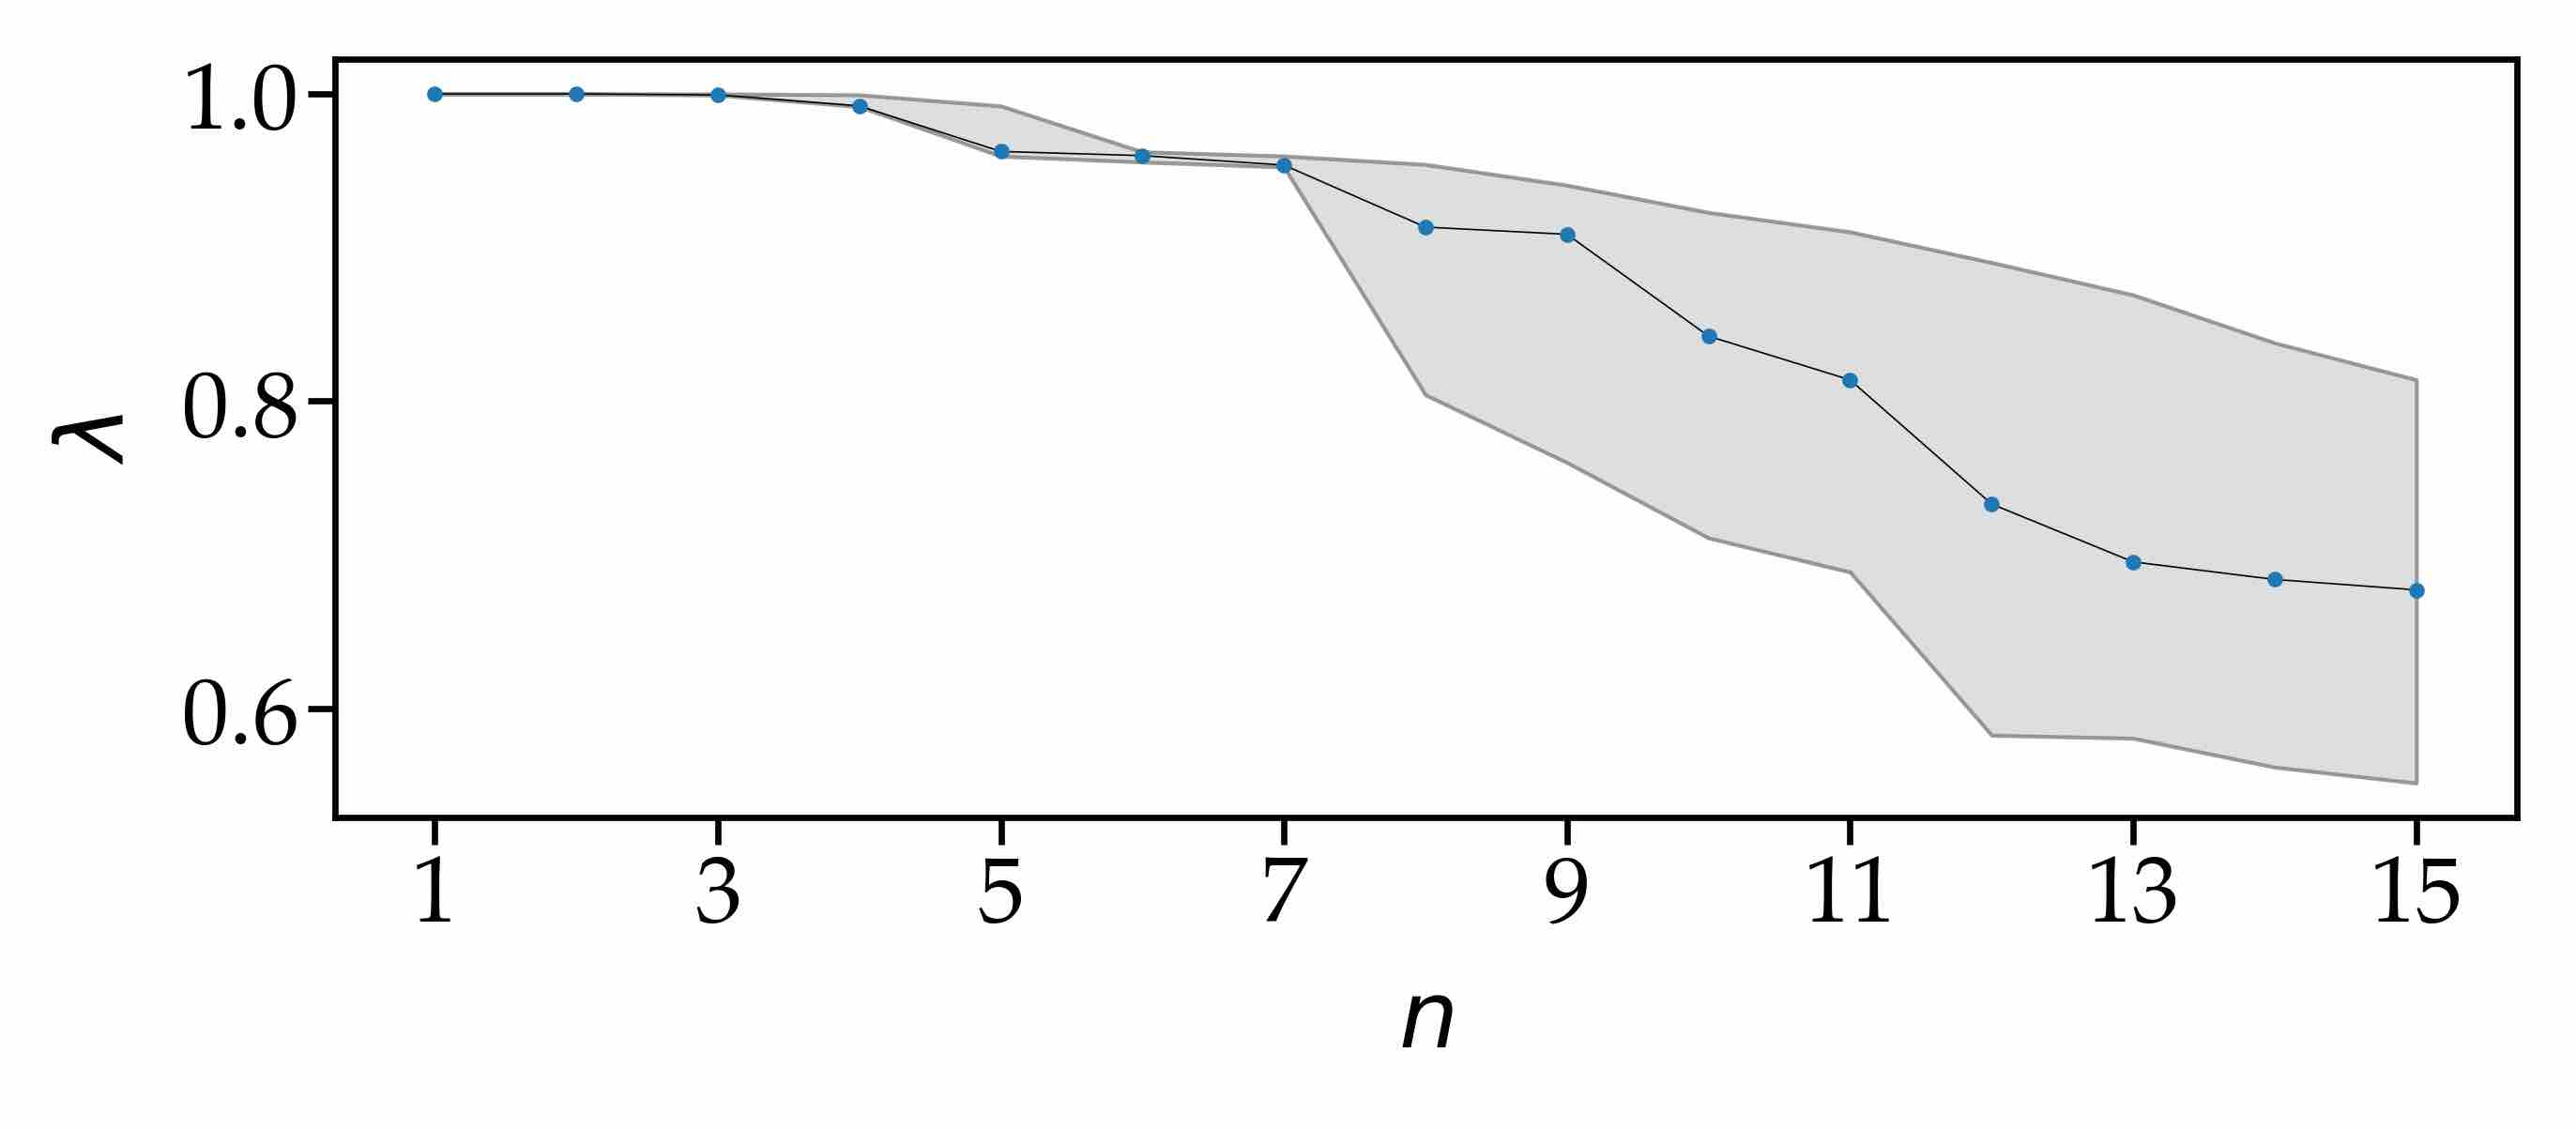
\includegraphics[width=\textwidth]{geogomdeep-fig06.jpg}
\end{figure}
}



\frame[allowframebreaks]{\frametitle{References}

% remove References title
\begingroup
\renewcommand{\section}[2]{}%
% add cited papers
\printbibliography[heading=none]
\endgroup
}

\end{document}